% =====================================================================
%  ARGUS CYCLIST: UM ECOSSISTEMA MULTIPLATAFORMA E DE CÓDIGO ABERTO
%  PARA O CICLISMO INDOOR
%  --------------------------------------------------------------------
%  Registro de Software — Trabalho de Conclusão de Curso
%  Autor: Paulo Sérgio Silva de Medeiros
%  Orientador: Prof. Dr. Isaac de Lima Oliveira Filho
%  Universidade do Estado do Rio Grande do Norte (UERN)
%  Curso de Bacharelado em Ciência da Computação
%
%  Para compilar (a partir desta pasta):
%     make                ou    latexmk -pdf main.tex
%  =====================================================================

\documentclass[
    a4paper,
    12pt,
    oneside,
    english,
    brazil,
    chapter=TITLE,
    section=TITLE,
]{abntex2}

% =========================== CONFIGURAÇÕES ==========================
% =====================================================================
%  PREÂMBULO DO DOCUMENTO
%  --------------------------------------------------------------------
%  Configuração da classe abntex2, pacotes, cores e hiperlinks.
%  =====================================================================

% ---------------------------------------------------------------------
%  Pacotes fundamentais
% ---------------------------------------------------------------------
\usepackage{cmap}                               % busca indexada no PDF
\usepackage[T1]{fontenc}                        % acentuação correta
\usepackage[utf8]{inputenc}                     % entrada UTF-8
\usepackage{lastpage}                           % referência à última página
\usepackage{graphicx}                           % figuras
\usepackage{xcolor}                             % cores
\usepackage{booktabs}                           % tabelas profissionais
\usepackage{multirow}                           % mescla células em tabelas
\usepackage{array}                              % colunas personalizadas
\usepackage{textcomp}                           % símbolos textuais
\usepackage{indentfirst}                        % indentação do 1º parágrafo
\usepackage{microtype}                          % microtipografia
\usepackage{amsmath,amssymb}                    % matemática
\usepackage{siunitx}                            % unidades SI
\usepackage{csquotes}                           % aspas tipográficas
\usepackage{pdfpages}                           % inclusão do certificado INPI

% ---------------------------------------------------------------------
%  TikZ — diagramas de arquitetura
% ---------------------------------------------------------------------
\usepackage{tikz}
\usetikzlibrary{arrows.meta,positioning,shapes.geometric,shapes.multipart,
  fit,calc,shadows,mindmap,trees,chains,scopes}

% ---------------------------------------------------------------------
%  Cores da identidade do Argus Cyclist
% ---------------------------------------------------------------------
\definecolor{blueargus}{RGB}{41, 98, 255}
\definecolor{greenargus}{RGB}{0, 200, 117}
\definecolor{orangeargus}{RGB}{255, 159, 10}
\definecolor{redargus}{RGB}{255, 69, 58}
\definecolor{darkbg}{RGB}{30, 30, 40}

% ---------------------------------------------------------------------
%  Hiperlinks
% ---------------------------------------------------------------------
\usepackage{hyperref}
\hypersetup{
    colorlinks=true,
    linkcolor=black,
    citecolor=black,
    urlcolor=blue,
}

% ---------------------------------------------------------------------
%  Citações no padrão ABNT (numérica)
% ---------------------------------------------------------------------
\usepackage[num]{abntex2cite}

% ---------------------------------------------------------------------
%  Tipografia
% ---------------------------------------------------------------------
\renewcommand{\familydefault}{\rmdefault}
\setlength{\parindent}{1.5cm}

% Espaçamento padrão ABNT (1,5) é definido pela classe abntex2.
% Para versão de rascunho com espaçamento simples, descomente:
% \singlespacing

% =====================================================================
%  COMANDOS PERSONALIZADOS
%  --------------------------------------------------------------------
%  \complementar{...}: destaca, no corpo do texto, trechos que ainda
%  precisam ser preenchidos pelo autor (não devem permanecer na versão
%  final). Ao finalizar o TCC, basta remover os chamados deste comando.
%  =====================================================================

% Caixa de destaque para informações a serem complementadas
\newcommand{\complementar}[1]{%
  \par\medskip\noindent
  \fcolorbox{red!70!black}{red!8}{%
    \begin{minipage}{\dimexpr\linewidth-2\fboxsep-2\fboxrule\relax}
      \textbf{\textcolor{red!80!black}{[COMPLEMENTAR]:}}~#1
    \end{minipage}%
  }\par\medskip
}

% Variante para uso dentro de células de tabela, parágrafos já abertos
% ou linhas de \assinatura (sem emitir \par/medskip no início e no fim).
\newcommand{\complementarcell}[1]{%
  \fcolorbox{red!70!black}{red!8}{%
    \begin{minipage}[c]{\dimexpr\linewidth-2\fboxsep-2\fboxrule\relax}
      \small\textbf{\textcolor{red!80!black}{[COMPLEMENTAR]:}}~#1
    \end{minipage}%
  }%
}

% Etiqueta compacta para células de tabela muito estreitas (sem caixa).
\newcommand{\complementartag}{%
  \textcolor{red!80!black}{\footnotesize\textbf{[COMPLEMENTAR]}}%
}

% Nota editorial genérica (subtítulo em versão de rascunho)
\newcommand{\rascunho}[1]{%
  \par\medskip\noindent
  \fcolorbox{gray}{gray!8}{%
    \begin{minipage}{\dimexpr\linewidth-2\fboxsep-2\fboxrule\relax}
      \textbf{\textcolor{gray}{[RASCUNHO]:}}~#1
    \end{minipage}%
  }\par\medskip
}

% Atalho para código com fonte monoespaçada
\newcommand{\code}[1]{\texttt{#1}}

% Nome realçado do projeto
\newcommand{\argus}{\textbf{Argus Cyclist}}

% =====================================================================
%  INFORMAÇÕES DO TRABALHO
%  --------------------------------------------------------------------
%  Edite aqui os dados institucionais e de autoria. Estes dados são
%  consumidos pela capa, folha de rosto, folha de aprovação e resumo.
%  =====================================================================

\instituicao{%
  Universidade do Estado do Rio Grande do Norte --- UERN
  \par
  Departamento de Informática --- Campus Central
  \par
  Curso de Bacharelado em Ciência da Computação
}

\tipotrabalho{Registro de Software}

\titulo{Argus Cyclist: um ecossistema multiplataforma e de código aberto para o ciclismo virtual}

\autor{Paulo Sérgio Silva de Medeiros}

\orientador[Prof. Dr.]{Isaac de Lima Oliveira Filho}

% Caso haja um professor da disciplina ou coorientador, descomente:
% \coorientador[Prof. Me.]{Antonio Oliveira Filho}

\local{Mossoró --- RN}

\data{2026}

\preambulo{Registro de software apresentado ao Curso de Bacharelado em Ciência da Computação da Universidade do Estado do Rio Grande do Norte --- UERN, como requisito para a obtenção do título de Bacharel em Ciência da Computação.}


% =========================== INÍCIO DO DOCUMENTO ====================
\begin{document}

% =========================== PRÉ-TEXTUAIS ============================
% =====================================================================
%  CAPA
% =====================================================================

\renewcommand{\imprimircapa}{%
  \begin{capa}
    \center
    \textbf{\large UNIVERSIDADE DO ESTADO DO RIO GRANDE DO NORTE}
    \par
    \textbf{DEPARTAMENTO DE INFORMÁTICA --- CAMPUS CENTRAL}
    \par
    \textbf{CURSO DE BACHARELADO EM CIÊNCIA DA COMPUTAÇÃO}
    \par
    \vspace{1.5cm}
    \textbf{\large PAULO SÉRGIO SILVA DE MEDEIROS}
    \vspace{4cm}
    \par
    \textbf{\Large ARGUS CYCLIST:}
    \par
    \textbf{\Large UM ECOSSISTEMA MULTIPLATAFORMA E DE CÓDIGO ABERTO}
    \par
    \textbf{\Large PARA O CICLISMO INDOOR}
    \vfill
    \textbf{MOSSORÓ --- RN}
    \par
    \textbf{2026}
  \end{capa}
}
\imprimircapa

% =====================================================================
%  FOLHA DE ROSTO
% =====================================================================

\begin{folhaderosto}
  \begin{center}
    \textbf{\large PAULO SÉRGIO SILVA DE MEDEIROS}
    \vspace{3.5cm}
    \par
    \textbf{\Large ARGUS CYCLIST:}
    \par
    \textbf{\Large UM ECOSSISTEMA MULTIPLATAFORMA E DE CÓDIGO ABERTO}
    \par
    \textbf{\Large PARA O CICLISMO INDOOR}
    \vspace{1.5cm}
    \par
    \hfill
    \begin{minipage}{0.45\textwidth}
      \small
      Registro de software apresentado ao Curso de Bacharelado em Ciência da
      Computação da Universidade do Estado do Rio Grande do Norte --- UERN,
      como requisito para a obtenção do título de Bacharel em Ciência da
      Computação.
      \vspace{0.5cm}
      \par
      \textbf{Orientador:} Prof. Dr. Isaac de Lima Oliveira Filho
    \end{minipage}
    \vfill
    \textbf{MOSSORÓ --- RN}
    \par
    \textbf{2026}
  \end{center}
\end{folhaderosto}

% =====================================================================
%  FOLHA DE APROVAÇÃO
%  --------------------------------------------------------------------
%  Banca preenchida. A data de aprovação deve ser informada após a
%  defesa.
%  =====================================================================

\begin{center}
  \textbf{\large PAULO SÉRGIO SILVA DE MEDEIROS}
  \vspace{1.2cm}
  \par
  \textbf{\Large ARGUS CYCLIST:}
  \par
  \textbf{\Large UM ECOSSISTEMA MULTIPLATAFORMA}
  \par
  \textbf{\Large E DE CÓDIGO ABERTO}
  \par
  \textbf{\Large PARA O CICLISMO VIRTUAL}
  \vspace{0.6cm}
  \par
  \hfill
  \begin{minipage}{0.52\textwidth}
    \small
    Trabalho de Conclusão de Curso apresentado como pré-requisito para a
    obtenção do título de Bacharel em Ciência da Computação da Universidade
    do Estado do Rio Grande do Norte --- UERN, submetido à aprovação da banca
    examinadora composta pelos seguintes membros:
  \end{minipage}
  \vspace{0.5cm}
  \par
  Aprovado em: \_\_\_\_/\_\_\_\_/\_\_\_\_
\end{center}

\vspace{2.3cm}

\noindent
\begin{minipage}[t]{0.48\textwidth}
  \centering
  \rule{6.4cm}{0.4pt}\\[0.15cm]
  \textbf{Prof. Dr. Isaac de Lima Oliveira Filho}\\
  (Orientador)\\
  Universidade do Estado do Rio Grande do Norte --- UERN
\vspace{2.5cm}
\end{minipage}\hfill
\begin{minipage}[t]{0.48\textwidth}
  \centering
  \rule{6.4cm}{0.4pt}\\[0.15cm]
  \textbf{Prof. Dr. Adalberto Veronese da Costa}\\
  Universidade do Estado do Rio Grande do Norte --- UERN
\vspace{2.5cm}
\end{minipage}

\vspace{1.0cm}

\noindent
\begin{minipage}[t]{0.48\textwidth}
  \centering
  \rule{6.4cm}{0.4pt}\\[0.15cm]
  \textbf{Prof. Me. Antonio Oliveira Filho}\\
  Universidade do Estado do Rio Grande do Norte --- UERN
\vspace{2.5cm}
\end{minipage}\hfill
\begin{minipage}[t]{0.48\textwidth}
  \centering
  \rule{6.4cm}{0.4pt}\\[0.15cm]
  \textbf{Prof. Dr. Sebastião Emidio Alves Filho}\\
  Universidade do Estado do Rio Grande do Norte --- UERN
\vspace{2.5cm}
\end{minipage}

\clearpage

% =====================================================================
%  PÁGINA DO REGISTRO DE SOFTWARE (INPI)
%  --------------------------------------------------------------------
%  Inclui o certificado oficial de registro do programa de computador
%  emitido pelo INPI (Processo nº BR512026003786-7), que representa a
%  versão inicial do software Argus Cyclist. A evolução da versão
%  registrada para a versão apresentada neste trabalho é detalhada no
%  Capítulo~\ref{cap:registro-evolucao}.
%  =====================================================================

\thispagestyle{empty}

\noindent
\begin{minipage}{\textwidth}
  \begin{center}
    \textbf{\large REGISTRO DE SOFTWARE --- INPI}
    \vspace{0.8cm}
  \end{center}

  O software \argus{} foi registrado junto ao Instituto Nacional da
  Propriedade Industrial (INPI) sob o Processo nº
  \textbf{BR512026003786-7}, sendo o registro expedido em 02/06/2026. O
  registro foi realizado com base na \textbf{versão inicial} do sistema,
  desenvolvida na etapa inicial do projeto. O presente trabalho apresenta a
  \textbf{evolução} do \argus{} desde essa versão registrada até a versão
  atual, documentando aprimoramentos, novas funcionalidades e a
  consolidação da arquitetura do sistema.
\end{minipage}

\vspace{0.6cm}

\centerline{%
  \fbox{%
    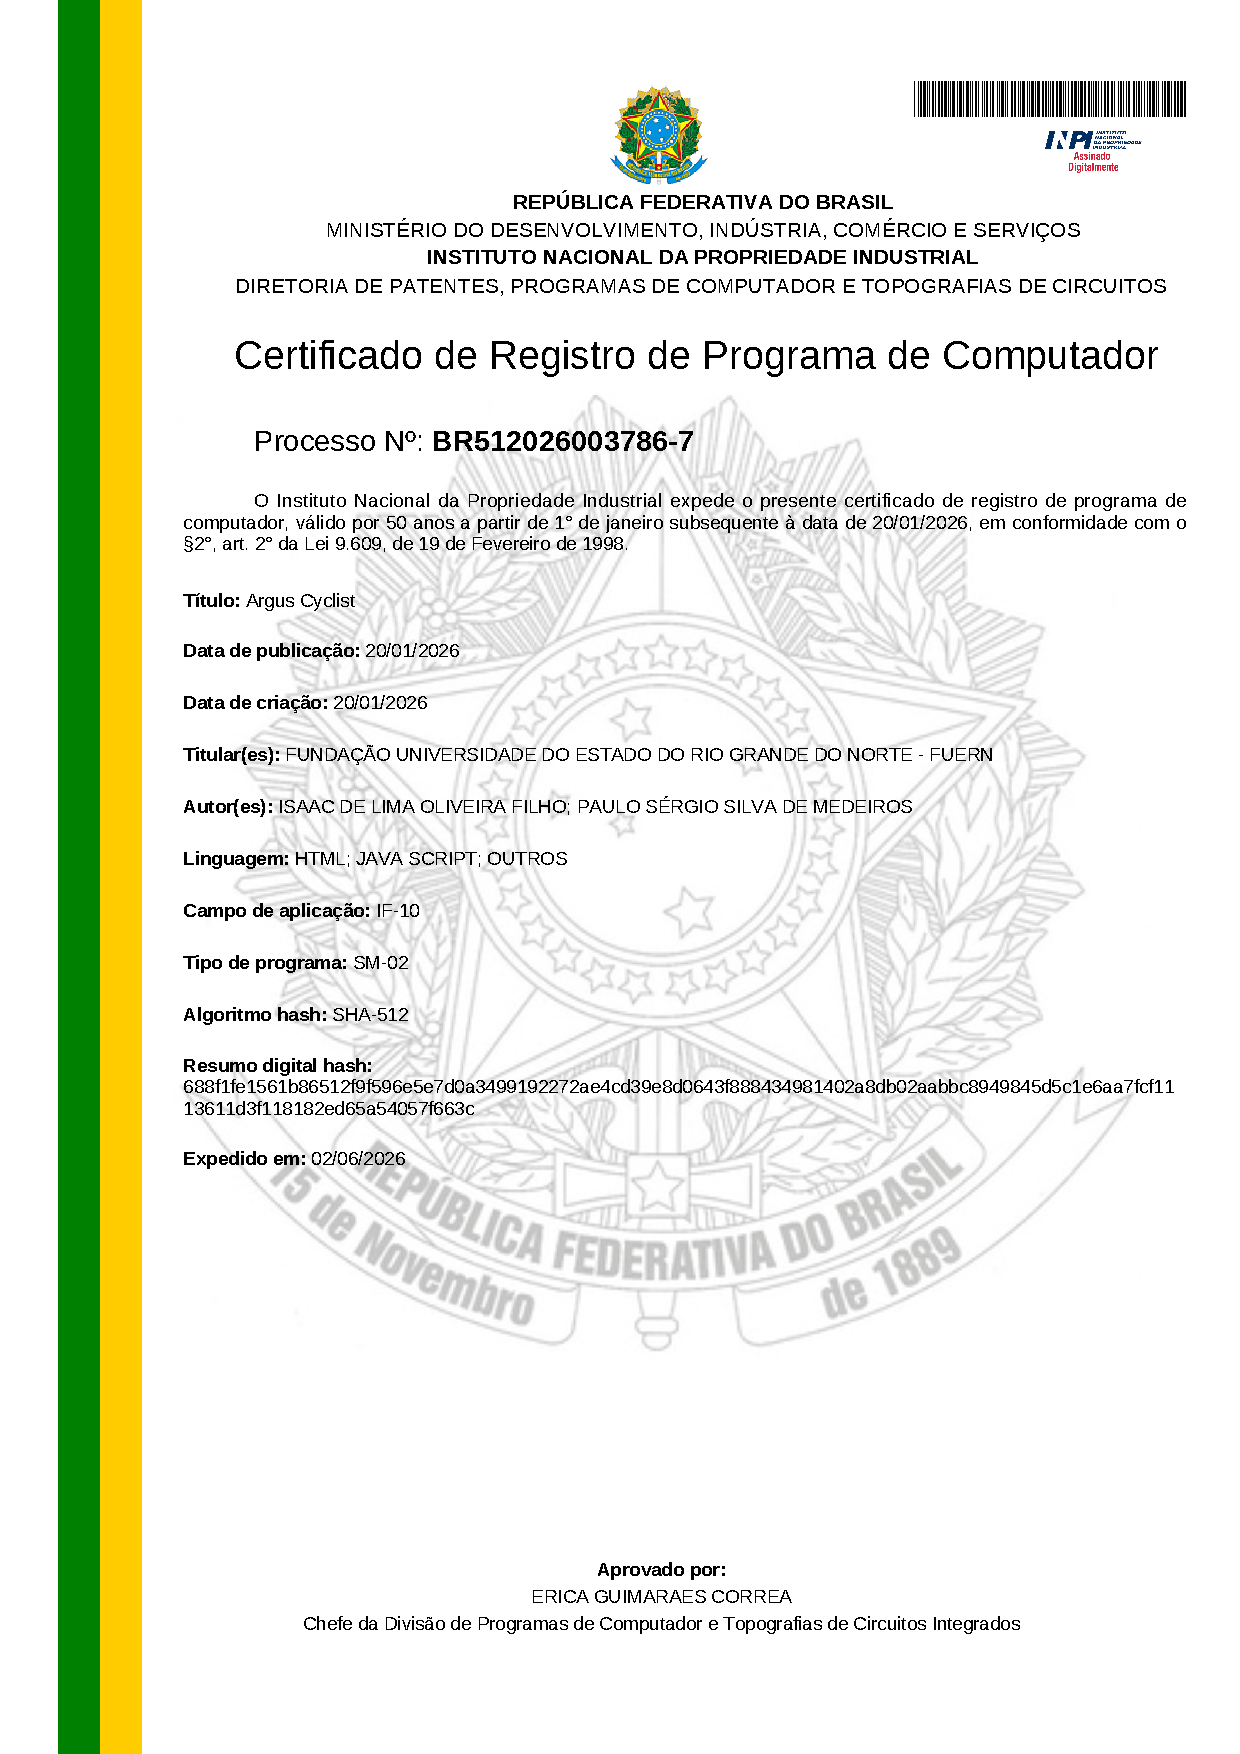
\includegraphics[width=0.75\textwidth,height=0.62\textheight,keepaspectratio]{certificado/certificado-registro-inpi.pdf}%
  }%
}

\vspace{0.6cm}

\begin{center}
  \small
  Certificado de Registro de Programa de Computador --- INPI
  \par
  Fonte: INPI (2026).
\end{center}

\newpage

% =====================================================================
%  RESUMO
% =====================================================================

\begin{resumo}

O ciclismo virtual combina rolos de treino inteligentes, simulação de percursos
e análise fisiológica, mas o fluxo de trabalho do ciclista costuma ser
fragmentado entre aplicativos de rota, treino e análise. Este trabalho
apresenta o \argus{}, um ecossistema de software multiplataforma e de código
aberto para simulação, exploração e análise de percursos reais no ciclismo
virtual. A tese que orienta o projeto é que o mesmo fluxo atende a quem vai
disputar uma prova e quer reconhecer o percurso, a quem quer conhecer e pedalar
um lugar que talvez nunca visite presencialmente e a quem quer treinar com
dados fisiológicos. O GPX entra, o rolo simula a estrada, a telemetria é
analisada e, no \textit{desktop}, o histórico permanece no dispositivo; no
Android, a sessão ao vivo cobre a importação, a simulação e a telemetria, sem
FIT ou histórico. O \textit{desktop} foi desenvolvido em Go, com interface
JavaScript embutida por meio do Wails; a mesma interface é reutilizada no
Android por meio do Capacitor, onde a física e o GPX são reimplementados em
JavaScript. O projeto adota princípios de \textit{Clean Architecture}, os
padrões \textit{Facade} e \textit{Repository} e persistência local em SQLite no
\textit{desktop}. A simulação física do \textit{desktop} utiliza a equação de
Martin para estimar a velocidade a partir da inclinação; o módulo de análise do
\textit{desktop} calcula Potência Normalizada (NP), Fator de Intensidade (IF),
\textit{Training Stress Score} (TSS), \textit{Training Impulse} (TRIMP),
\textit{Performance Management Chart} (PMC), recuperação da frequência cardíaca
(HRR) e desacoplamento cardiovascular, com fórmulas e limitações documentadas.
O trabalho adota a \textit{Design Science Research} e avalia o artefato por meio
de um estudo piloto com o próprio autor, complementado por testes de integração
e de exportação de arquivos \texttt{.FIT}. Foram validados o \textit{desktop}
Windows/Linux no fluxo completo e o telefone Android em sessão ao vivo;
iOS/iPadOS, tablet Android e \textit{desktop} macOS permanecem como preparação
arquitetural ou layout projetado, sem validação em dispositivo. O código é distribuído sob GPLv3 e o registro da
versão inicial foi depositado no Instituto Nacional da Propriedade Industrial
(INPI, Processo BR512026003786-7).

\textbf{Palavras-chave}: Ciclismo virtual. Percursos reais. Código aberto.
Análise fisiológica. Multiplataforma. \textit{Design Science Research}.

\end{resumo}

% =====================================================================
%  ABSTRACT
% =====================================================================

\begin{resumo}[Abstract]
\begin{otherlanguage*}{english}

Virtual cycling has become a sport modality recognized by the Union
Cycliste Internationale (UCI), yet access to simulation platforms is
restricted by monthly subscription fees in foreign currency, high-performance
hardware requirements, and continuous internet dependence. This work presents
the software registration of Argus Cyclist, an open-source cross-platform
virtual cycling simulator licensed under GPLv3, developed in Go (Golang) with
a JavaScript frontend using the Wails framework for desktop and Capacitor.js
for Android mobile devices. The system employs a Clean Architecture with
Facade and Repository patterns, abstracting Bluetooth Low Energy (BLE)
connections for heart rate, power, and smart trainer control via GATT profiles
(\texttt{0x180D}, \texttt{0x1818}, \texttt{0x1826}). The physics engine
implements Martin's equation for speed calculation from GPX route gradients,
while the physiological analysis module computes advanced metrics such as
Normalized Power (NP), Training Stress Score (TSS), Performance Management
Chart (PMC), and Aerobic Decoupling. It distinguishes itself by incorporating
a local generative AI coaching assistant (Ollama) for creating personalized
workout plans in ZWO format, along with a bicycle component wear tracking
system. The software was registered at the Brazilian National Institute of
Industrial Property (INPI, Process BR512026003786-7) in its initial version,
having evolved significantly after the registration with new modules, training
modes, third-party integrations, and architecture improvements. Experimental
validation uses real cycling equipment to verify telemetry latency below
\SI{150}{\milli\second} and \texttt{.fit} file compliance with the Garmin
standard. The project aims to democratize scientific high-performance training
by eliminating economic and connectivity barriers.

\textbf{Keywords}: Virtual cycling. Open source. Physics simulation. Bluetooth
Low Energy. Physiological analysis. Artificial intelligence.

\end{otherlanguage*}
\end{resumo}

% =====================================================================
%  LISTAS PRÉ-TEXTUAIS
%  (figuras, tabelas, siglas e abreviaturas)
% =====================================================================

% ---------------------------------------------------------------------
%  Lista de ilustrações (figuras)
% ---------------------------------------------------------------------
\pdfbookmark[0]{\listfigurename}{lof}
\listoffigures*
\clearpage

% ---------------------------------------------------------------------
%  Lista de tabelas
% ---------------------------------------------------------------------
\pdfbookmark[0]{\listtablename}{lot}
\listoftables*
\clearpage

% ---------------------------------------------------------------------
%  Lista de siglas e abreviaturas
% ---------------------------------------------------------------------
\begin{siglas}
    \item[ATL] \textit{Acute Training Load} (Carga de Treino Aguda)
    \item[BLE] \textit{Bluetooth Low Energy}
    \item[CTL] \textit{Chronic Training Load} (Carga de Treino Crônica)
    \item[ERG] \textit{Ergometer Mode} (Modo Ergômetro)
    \item[FTP] \textit{Functional Threshold Power} (Potência Funcional Limiar)
    \item[FTMS] \textit{Fitness Machine Service}
    \item[GATT] \textit{Generic Attribute Profile}
    \item[GPX]  \textit{GPS Exchange Format}
    \item[HRR]  \textit{Heart Rate Recovery} (Recuperação da Frequência Cardíaca)
    \item[IF]   \textit{Intensity Factor} (Fator de Intensidade)
    \item[INPI] Instituto Nacional da Propriedade Industrial
    \item[IPC]  \textit{Inter-Process Communication}
    \item[KOM]  \textit{King of the Mountain}
    \item[LLM]  \textit{Large Language Model}
    \item[NP]   \textit{Normalized Power} (Potência Normalizada)
    \item[PMC]  \textit{Performance Management Chart}
    \item[PR]   \textit{Personal Record}
    \item[SDK]  \textit{Software Development Kit}
    \item[SQL]  \textit{Structured Query Language}
    \item[TSB]  \textit{Training Stress Balance} (Balanço de Estresse de Treino)
    \item[TSS]  \textit{Training Stress Score}
    \item[UCI]  \textit{Union Cycliste Internationale} (União Ciclística Internacional)
    \item[UI]   \textit{User Interface} (Interface de Usuário)
    \item[XP]   \textit{Experience Points} (Pontos de Experiência)
    \item[ZWO]  \textit{Zwift Workout}
\end{siglas}

\clearpage

% =====================================================================
%  SUMÁRIO
% =====================================================================

\pdfbookmark[0]{\contentsname}{toc}
\tableofcontents*
\clearpage


% =========================== TEXTUAIS ================================
\textual

% =====================================================================
%  CAPÍTULO 1 — INTRODUÇÃO
% =====================================================================

\chapter{INTRODUÇÃO}
\label{cap:introducao}

O ciclismo virtual (\textit{indoor cycling}) transitou de uma simples
atividade alternativa para dias chuvosos para uma modalidade esportiva e
científica de alta relevância global. Atualmente, é reconhecida pela União
Ciclística Internacional (UCI) como uma modalidade oficial de
\textit{e-sports}, contando com campeonatos mundiais e atletas profissionais
dedicados \cite{coggan2010}. Este fenômeno foi impulsionado pelo surgimento de
rolos de treino inteligentes (\textit{smart trainers}), capazes de estabelecer
comunicação bidirecional com computadores e dispositivos móveis para simular a
resistência do terreno real em tempo real.

No entanto, a situação atual do ciclismo virtual é marcada por uma forte
centralização de mercado e barreiras econômicas severas. Plataformas líderes
como Zwift, Rouvy e TrainerRoad operam sob modelos de assinatura mensal
proprietários com taxas cobradas em dólar comercial, em torno de
\$20~USD/mês. Para atletas em países em desenvolvimento, como o Brasil, o
custo acumulado dessas assinaturas ultrapassa R\$~1.200,00 anuais (em média
\$240~USD/ano no plano mensal), o que constitui um fator de exclusão para
ciclistas amadores e atletas de base.

Além da barreira financeira, essas plataformas comerciais exigem hardware de
alto desempenho com placas gráficas dedicadas, inviabilizando o uso por
atletas que possuem apenas computadores de entrada ou dispositivos móveis
comuns. Adicionalmente, tais soluções dependem de conexão contínua com a
internet para computar métricas, o que impede treinos em ambientes
\textit{offline} ou com conectividade instável.

O \argus{} propõe-se a ser uma alternativa nacional, multiplataforma,
\textit{offline-first} e de código aberto, unindo simulação física interativa,
telemetria de precisão, assistência de inteligência artificial generativa
local e rastreamento de desgaste de componentes, sem taxas recorrentes e com
baixíssimos requisitos de hardware. Este documento constitui o registro do
software desenvolvido, apresentando sua arquitetura, implementação, resultados
e a evolução do projeto desde a versão registrada junto ao INPI.

\section{Contextualização: a situação atual do ciclismo virtual}
\label{sec:contextualizacao}

A seção a seguir apresenta o estado da arte do ciclismo virtual, comparando o
\argus{} com as principais plataformas do mercado e iniciativas de código
aberto, para situar o leitor quanto ao contexto tecnológico e mercadológico no
qual o software se insere.

\subsection{Estado da arte e referências a outros projetos}
\label{sec:estado-arte}

Para contextualizar a relevância e o posicionamento do \argus{}, apresenta-se
a seguir um comparativo com as principais plataformas do mercado e iniciativas
de código aberto:

\begin{itemize}
    \item \textbf{Zwift}: o líder absoluto do mercado foca em um ambiente
        virtual tridimensional massivo \textit{online}, com forte apelo social
        e gamificação. Suas limitações residem na ausência de modo
        \textit{offline}, custo recorrente elevado (\$19,99~USD/mês) e exigência
        de hardware potente para processamento gráfico 3D.
    \item \textbf{Rouvy}: diferencia-se por simular rotas reais por meio de
        vídeos gravados de estradas ao redor do mundo. Apresenta alta demanda
        de largura de banda de rede para transmissão de vídeo e sofre dos
        mesmos problemas de custo de assinatura fechada (\$19,99~USD/mês).
    \item \textbf{TrainerRoad}: foca exclusivamente em treinos estruturados
        baseados em faixas de potência (telemetria pura), sem simulação
        gráfica complexa. Suas métricas e planos de treino são proprietários e
        bloqueados por assinaturas de custo elevado (\$19,95~USD/mês).
    \item \textbf{GoldenCheetah}: software livre sob licença GPLv3 voltado à
        análise científica pós-treino. Embora possua ferramentas matemáticas
        excelentes (como o gráfico PMC e modelos de fadiga), sua interface é
        extremamente complexa, com uma curva de aprendizado íngreme, e ele não
        foi projetado para atuar como um simulador de rotas interativo e
        responsivo em tempo real com controle de rolos inteligentes.
    \item \textbf{Argus Cyclist}: posiciona-se no estado da arte ao preencher
        a lacuna entre a análise de dados científica (típica do GoldenCheetah)
        e a simulação de rotas interativa e gamificada (típica do Zwift),
        operando de forma totalmente gratuita, multiplataforma,
        \textit{offline-first} e com processamento local eficiente.
        Diferencia-se ainda por oferecer um treinador virtual baseado em IA
        generativa local (Ollama) \cite{ollama2024} para elaboração de treinos
        personalizados em linguagem natural e um sistema de rastreamento de
        desgaste de componentes que calcula automaticamente a vida útil
        restante de cada peça da bicicleta com base na distância percorrida.
\end{itemize}

\begin{table}[h]
    \centering
    \caption{Comparativo entre plataformas de ciclismo virtual}
    \label{tab:comparativo}
    \small
    \begin{tabular}{
        >{\raggedright\arraybackslash}p{2.8cm}
        >{\raggedright\arraybackslash}p{2.4cm}
        >{\raggedright\arraybackslash}p{2.2cm}
        >{\raggedright\arraybackslash}p{2cm}
        >{\centering\arraybackslash}p{1.1cm}
        >{\raggedright\arraybackslash}p{3cm}
    }
        \toprule
        \textbf{Plataforma} & \textbf{Licença} & \textbf{Execução} &
        \textbf{Hardware} & \textbf{Offline} & \textbf{Foco Principal} \\
        \midrule
        Zwift & Proprietária (\$19,99/mês) & Nuvem & Alto & Não &
        Gamificação e Social \\
        Rouvy & Proprietária (\$19,99/mês) & Nuvem & Médio-Alto & Não &
        Realismo de rotas reais \\
        TrainerRoad & Proprietária (\$19,95/mês) & Nuvem & Baixo & Não &
        Treinos Estruturados \\
        GoldenCheetah & Livre (GPLv3) & Local & Baixo & Sim &
        Análise Científica pós-treino \\
        \textbf{Argus Cyclist} & \textbf{Livre (GPLv3)} &
        \textbf{Local (Edge)} & \textbf{Baixo} & \textbf{Sim} &
        \textbf{Física + Telemetria + IA} \\
        \bottomrule
    \end{tabular}
\end{table}

\section{Problemática}
\label{sec:problematica}

O desenvolvimento do projeto \argus{} é motivado por quatro problemas centrais
identificados no ecossistema atual do ciclismo virtual:

\begin{enumerate}
    \item \textbf{Exclusão socioeconômica e barreiras de acesso}: o modelo de
        monetização em moeda estrangeira das plataformas de \textit{e-sports}
        de ciclismo inviabiliza o treinamento científico e estruturado para
        atletas de base e ciclistas amadores de menor poder aquisitivo no
        Brasil.

    \item \textbf{Dependência crônica de conectividade (\textit{cloud lock-in})}:
        a arquitetura das soluções comerciais centraliza a lógica do simulador
        e o processamento de métricas em servidores na nuvem. Quedas temporárias
        de conexão resultam no encerramento abrupto das atividades ou na perda
        de treinos inteiros, além de inviabilizar o uso em locais sem sinal de
        internet.

    \item \textbf{Vulnerabilidade de privacidade de dados}: a coleta de dados
        biométricos (frequência cardíaca contínua) e geográficos (coordenadas
        GPS de rotas importadas) é armazenada de forma compulsória em
        servidores privados estrangeiros, infringindo princípios de soberania
        de dados e privacidade por padrão (\textit{Privacy-by-Design}).

    \item \textbf{Monetização fisiológica abusiva}: métricas avançadas de
        controle de carga de treinos fundamentais para evitar o
        \textit{overtraining} e prescrever a recuperação (como PMC, TSS e CTL)
        dependem apenas de equações matemáticas consolidadas na literatura
        científica de fisiologia do esporte. Ainda assim, são vendidas como
        recursos exclusivos em softwares proprietários pagos.
\end{enumerate}

\section{Justificativa}
\label{sec:justificativa}

O projeto \argus{} justifica-se pela sua contribuição tecnológica, científica
e de impacto social no cenário esportivo e de engenharia de software.

\subsection{Relevância tecnológica e inovação arquitetural}
\label{sec:relevancia-tecnologica}

Do ponto de vista da Engenharia de Software, o projeto aborda o desafio de
criar um sistema multiplataforma de tempo real de baixíssima latência. A
escolha do Go (Golang) no \textit{backend} deve-se à sua capacidade nativa de
concorrência baseada em \textit{goroutines} e \textit{channels}, permitindo
realizar escaneamento e manter conexões estáveis com múltiplos sensores
Bluetooth Low Energy (BLE) utilizando a biblioteca TinyGo Bluetooth
\cite{tinygo2024} com perfis GATT específicos (frequência cardíaca
\cite{bluetooth2017}, potência e controle bidirecional FTMS) sem congelar a
interface de usuário.

A integração com o framework Wails \cite{wails2024} viabiliza um binário de
\textit{desktop} extremamente leve, utilizando a \textit{web engine} nativa do
sistema operacional para renderizar uma interface reativa em JavaScript
(Vite), registrando um consumo de memória inferior a \SI{200}{\mega\byte} ---
uma fração do demandado por soluções baseadas em Electron. Para dispositivos
móveis, a utilização do Capacitor.js \cite{capacitor2024} possibilita
reutilizar a mesma base de código do \textit{frontend} para compilar um
aplicativo nativo para Android, rodando um motor físico portado inteiramente
para JavaScript para simular e controlar os rolos diretamente de um celular
comum via antenas BLE integradas.

Inovadoramente, o sistema incorpora um módulo de IA generativa local que se
comunica com uma instância do Ollama \cite{ollama2024} rodando no próprio
dispositivo do usuário. Esta arquitetura elimina completamente a dependência de
serviços em nuvem para funcionalidades de \textit{coaching}, garantindo que
nenhum dado biométrico ou de treino seja transmitido a servidores externos. A
escolha de modelos pequenos (três bilhões de parâmetros, como o
\texttt{qwen2.5:3b}) viabiliza a execução mesmo em hardware modesto, e o tempo
de resposta estendido acomoda a inferência em CPU.

O sistema de controle de desgaste de componentes implementa um modelo de
depreciação linear simples, porém eficaz, onde cada componente cadastrado
(corrente, cassete, coroas, etc.) tem sua vida útil definida em quilômetros
pelo usuário, e o desgaste percentual é atualizado automaticamente ao final de
cada sessão de treino com base na distância percorrida. Este sistema segue uma
arquitetura em camadas bem definida com persistência em SQLite
\cite{sqlite2024} local, mantendo a coerência com o princípio
\textit{offline-first} do projeto.

\subsection{Relevância científica (modelagem física e fisiologia)}
\label{sec:relevancia-cientifica}

O sistema aplica modelagens matemáticas rigorosas de física e fisiologia do
esporte diretamente no dispositivo do usuário. O motor físico calcula a
aceleração e a velocidade virtual aplicando a conservação de energia sobre as
forças resistivas, conforme a equação de Martin \cite{martin1998}, detalhada
no Capítulo~\ref{cap:fundamentacao}. O módulo de fisiologia processa o vetor de
potência de \SI{1}{\hertz} para extrair métricas como Potência Normalizada
(NP), Fator de Intensidade (IF), \textit{Training Stress Score} (TSS),
\textit{Training Impulse} (TRIMP), além de compilar o
\textit{Performance Management Chart} (PMC) e o desvio cardiovascular
(\textit{Aerobic Decoupling}), fundamentadas na literatura de fisiologia do
esporte \cite{coggan2010}.

\subsection{Relevância social e inclusão esportiva}
\label{sec:relevancia-social}

Ao prover uma solução \textit{offline} de código aberto e totalmente gratuita
compatível com computadores modestos e celulares Android, o \argus{} atua como
um elemento de inclusão social. O projeto permite que ciclistas locais e
equipes amadoras de ciclismo utilizem equipamentos de rolo de treino
inteligente sem taxas mensais, democratizando o treinamento esportivo de alto
rendimento.

\section{Objetivos}
\label{sec:objetivos}

\subsection{Objetivo geral}
\label{sec:objetivo-geral}

Projetar, desenvolver e validar o \argus{}, um simulador multiplataforma de
ciclismo virtual de código aberto e gratuito, integrado a um sistema científico
de análise de telemetria esportiva \textit{offline-first}, garantindo
processamento em borda (\textit{edge}) de baixa latência e interoperabilidade
com hardware padrão do mercado.

\subsection{Objetivos específicos}
\label{sec:objetivos-especificos}

\begin{enumerate}
    \item \textbf{Conectividade de hardware}: implementar rotinas robustas em
        Go para escaneamento e conexão com periféricos via Bluetooth Low
        Energy (BLE), decodificando serviços GATT para cintas cardíacas
        (\texttt{0x180D}), sensores de potência (\texttt{0x1818}) e rolos de
        treino controlados (FTMS --- \texttt{0x1826}) \cite{bluetooth2017}.
    \item \textbf{Motor de simulação física}: desenvolver algoritmos que
        traduzam o gradiente das coordenadas de uma rota GPX
        \cite{gpx2004} em resistência de torque mecânico no rolo de treino
        inteligente, atualizando dinamicamente a resistência conforme o peso do
        ciclista e sua inclinação virtual.
    \item \textbf{Interface gráfica de alta performance}: construir um HUD
        (\textit{Heads-Up Display}) leve a 60~fps usando Canvas/WebGL,
        integrando o MapLibre GL JS \cite{maplibre2024} com renderização
        topográfica em 3D Terrain-RGB e rotas dinâmicas coloridas de acordo
        com a inclinação do terreno.
    \item \textbf{Análise fisiológica local}: implementar funções matemáticas
        para cálculo contínuo de métricas esportivas avançadas (NP, IF, TSS,
        TRIMP) e visualização do gráfico de evolução histórica de carreira PMC
        (\textit{Performance Management Chart}).
    \item \textbf{Assistente de treino por IA generativa local (IA Coach)}:
        integrar um assistente conversacional de treinamento esportivo
        utilizando modelos de linguagem de pequena escala (3B parâmetros)
        executados localmente via Ollama \cite{ollama2024}, capaz de
        interpretar o perfil do atleta e gerar planos de treino estruturados no
        formato ZWO (\textit{Zwift Workout}) com carregamento automático no
        modo ERG do simulador.
    \item \textbf{Controle de desgaste de componentes mecânicos}: implementar
        um sistema de cadastro e monitoramento de componentes da bicicleta com
        cálculo automático de desgaste percentual baseado na quilometragem
        acumulada, histórico de substituições com auditoria temporal e
        indicadores visuais codificados por cores (verde, amarelo, vermelho)
        para alertar o atleta sobre a necessidade de manutenção preventiva.
    \item \textbf{Persistência de dados confiável}: modelar um banco de dados
        local com SQLite \cite{sqlite2024} usando os padrões
        \textit{Repository} e \textit{Facade} para persistir usuários,
        atividades e recordes pessoais de forma 100\% \textit{offline} e
        estruturada.
    \item \textbf{Interoperabilidade de dados}: desenvolver rotinas para
        compilação e exportação de dados na estrutura de arquivo binário
        padrão \texttt{.FIT} (Garmin/ANT+ SDK) \cite{garmin2024} e integração
        de upload assíncrono via API do Strava \cite{strava2025} e do
        Intervals.icu \cite{intervals2024}.
    \item \textbf{Portabilidade multiplataforma}: compilar a aplicação para os
        sistemas Android, Windows, macOS e Linux utilizando tecnologias
        multiplataforma, adaptando o motor físico para JavaScript a fim de
        garantir operação autônoma, compatibilidade entre diferentes ambientes
        e baixa latência em dispositivos móveis e \textit{desktops}.
    \item \textbf{Gamificação saudável}: integrar um sistema de níveis e
        conquistas cardiovasculares persistentes com uma \textit{Trophy Room}
        interativa 3D/Canvas para engajamento dos atletas amadores.
\end{enumerate}

\section{Metodologia}
\label{sec:metodologia}

O trabalho adota uma metodologia de pesquisa aplicada, orientada ao
desenvolvimento tecnológico experimental, utilizando abordagens qualitativas e
quantitativas para validação dos resultados. O processo de engenharia de
software baseia-se em um modelo de desenvolvimento iterativo e incremental
(práticas ágeis), dividido em quatro fases essenciais.

\subsection{Fases do desenvolvimento}
\label{sec:fases}

\begin{enumerate}
    \item \textbf{Fase de levantamento e especificação}: estudo aprofundado dos
        perfis GATT Bluetooth SIG (\textit{Heart Rate Service},
        \textit{Cycling Power Service} e \textit{Fitness Machine Service}) e
        decodificação hexadecimal de \textit{frames} de telemetria. Análise da
        documentação do Garmin FIT SDK \cite{garmin2024} para modelar o
        codificador de arquivos binários e das APIs REST do Strava sob
        protocolo de segurança OAuth 2.0 \cite{strava2025}.

    \item \textbf{Fase de definição arquitetural}: desenho do padrão estrutural
        do sistema sob conceitos de \textit{Clean Architecture}. Separação
        rígida de responsabilidades em camadas (Apresentação, Casos de Uso,
        Serviços de Domínio e Persistência de Dados). Seleção da \textit{stack}
        multiplataforma ideal: \textit{backend} em Go (Golang) com
        \textit{bindings} Wails (Desktop) e empacotamento móvel nativo em
        Android via Capacitor.js \cite{capacitor2024}.

    \item \textbf{Fase de implementação e refatoração}: implementação dos
        serviços em Go: módulo de telemetria (\code{internal/service/ble}) com
        \textit{goroutines} concorrentes de escuta; módulo físico
        (\code{internal/service/sim}) com suporte a GPX e testes de FTP;
        persistência em banco local (\code{internal/repository/sqlite}) sob
        padrão \textit{Facade} (\code{usecase/storage\_facade}); e exportador
        esportivo (\code{internal/service/fit}). No \textit{frontend}
        JavaScript, implementa-se o \code{TelemetryEventBus} para desacoplar a
        atualização de tela da chegada de dados BLE, garantindo renderização
        fluida a 60~fps.

    \item \textbf{Fase de testes e validação experimental}: execução de testes
        funcionais e de integração utilizando equipamentos reais de ciclismo,
        conectando o \argus{} a rolos inteligentes (\textit{smart trainers}) e
        medidores de potência para validação prática do sistema em ambiente de
        uso real. A validação quantitativa consiste na medição da latência de
        telemetria (requisitada para operar em $<$ \SI{150}{\milli\second} do
        hardware até a tela) e em testes de conformidade estrutural,
        submetendo os arquivos binários \texttt{.fit} gerados diretamente ao
        Strava \cite{strava2025}, atestando a integridade estatística dos
        dados em relação ao padrão global da indústria.
\end{enumerate}

Dessa forma, a metodologia proposta garante a consistência científica no
desenvolvimento e assegura a qualidade física da simulação interativa,
resultando em um produto de software estável e utilizável por ciclistas.

\section{Organização do documento}
\label{sec:organizacao}

Este documento está organizado da seguinte forma: o Capítulo~\ref{cap:introducao}
apresenta a contextualização, problemática, justificativa, objetivos e
metodologia; o Capítulo~\ref{cap:fundamentacao} apresenta a fundamentação
teórica necessária à compreensão do sistema; o Capítulo~\ref{cap:registro-evolucao}
contextualiza o registro do software junto ao INPI e documenta a evolução do
projeto desde a versão registrada; o Capítulo~\ref{cap:arquitetura} descreve a
arquitetura do sistema; o Capítulo~\ref{cap:implementacao} detalha a
implementação dos módulos e funcionalidades; o Capítulo~\ref{cap:resultados}
apresenta os resultados e a validação do software; e o Capítulo~\ref{cap:conclusao}
tece as considerações finais e trabalhos futuros.

% =====================================================================
%  CAPÍTULO 2 — FUNDAMENTAÇÃO TEÓRICA
% =====================================================================

\chapter{FUNDAMENTAÇÃO TEÓRICA}
\label{cap:fundamentacao}

Este capítulo apresenta os conceitos teóricos necessários à compreensão do
\argus{}, abrangendo desde os protocolos de comunicação sem fio de baixo
consumo até os modelos físicos e fisiológicos utilizados no cálculo de
telemetria, bem como os princípios de engenharia de software que guiam a
arquitetura do sistema.

\section{Bluetooth Low Energy e perfis GATT}
\label{sec:ble-gatt}

O \textit{Bluetooth Low Energy} (BLE) é uma tecnologia de comunicação sem fio
de curto alcance e baixo consumo energético, projetada para dispositivos que
necessitam transmitir pequenas quantidades de dados de forma intermitente,
como sensores esportivos \cite{bluetooth2017}. No contexto do ciclismo, sensores
de frequência cardíaca, medidores de potência e rolos de treino inteligentes
utilizam o BLE para transmitir telemetria em tempo real.

O \textit{Generic Attribute Profile} (GATT) define a estrutura de dados sobre a
qual os serviços são expostos. Cada serviço é identificado por um UUID e contém
características (\textit{characteristics}) que podem ser lidas, escritas ou
assinar notificações. Os serviços relevantes ao \argus{} são:

\begin{itemize}
    \item \textbf{Heart Rate Service} (\texttt{0x180D}): expõe a frequência
        cardíaca instantânea do atleta, geralmente em batimentos por minuto
        (BPM) \cite{bluetooth2017}.
    \item \textbf{Cycling Power Service} (\texttt{0x1818}): transmite a
        potência instantânea (em watts) e, opcionalmente, cadência e
        distribuição do torque aplicado aos pedais.
    \item \textbf{Fitness Machine Service} (FTMS, \texttt{0x1826}): permite o
        controle bidirecional de equipamentos de fitness, incluindo a leitura
        de telemetria do rolo e o envio de comandos de resistência, habilitando
        modos como ERG (potência alvo fixa) e simulação de inclinação
        \cite{bluetooth2017}.
\end{itemize}

Além do FTMS, rolos de treino de diferentes fabricantes podem expor o protocolo
FE-C (ANT+), que também é suportado pelo \argus{} para controle de resistência
em modos ERG e de altitude simulada.

\section{Protocolos e formatos de dados esportivos}
\label{sec:formatos}

\subsection{GPX (\textit{GPS Exchange Format})}
\label{sec:gpx}

O GPX é um formato aberto baseado em XML, criado pela Topografix, para o
intercâmbio de dados de posicionamento geográfico (latitude, longitude e
elevação) \cite{gpx2004}. No \argus{}, rotas GPX são importadas para extrair o
perfil de elevação e, a partir da diferença de altitude entre pontos
consecutivos, calcular o gradiente percentual da via, que alimenta o motor de
simulação física.

\subsection{FIT (\textit{Flexible and Interoperable Data Transfer})}
\label{sec:fit}

O formato FIT, especificado pela Garmin e pela aliança ANT+, é um formato
binário compacto e interoperável para armazenamento de atividades esportivas
\cite{garmin2024}. Arquivos FIT são amplamente aceitos por plataformas como
Strava, Garmin Connect e TrainingPeaks. O \argus{} gera arquivos FIT ao final
de cada sessão, permitindo que os treinos sejam importados por essas
plataformas sem conversão.

\subsection{ZWO (\textit{Zwift Workout})}
\label{sec:zwo}

O ZWO é o formato de plano de treino estruturado utilizado pela plataforma
Zwift, definindo intervalos com duração e alvo de potência (em percentual do
FTP) em modo ERG \cite{zwift2024}. O \argus{} importa e gera arquivos ZWO,
permitindo que planos de treino elaborados pelo assistente de IA sejam
carregados diretamente no simulador.

\section{Modelagem física do ciclismo: a equação de Martin}
\label{sec:equacao-martin}

O movimento de uma bicicleta pode ser modelado pelo balanço de forças que
atuam sobre o conjunto ciclista--bicicleta. O modelo proposto por Martin
\cite{martin1998} relaciona a potência aplicada pelo ciclista ($P$) à
velocidade ($v$), considerando as forças de arrasto aerodinâmico, resistência
ao rolamento, componente gravitacional do gradiente e aceleração linear,
conforme a Equação~\ref{eq:martin}:

\begin{equation}\label{eq:martin}
P = v \cdot \left( \frac{1}{2} \rho C_d A \, v^2 + m g C_{rr} + m g \sin\theta + m a \right) \cdot \eta^{-1}
\end{equation}

\noindent em que:
\begin{itemize}
    \item $\rho$ é a densidade do ar (\SI{1,225}{\kilo\gram\per\cubic\meter}
        ao nível do mar);
    \item $C_d A$ é o coeficiente de arrasto aerodinâmico multiplicado pela
        área frontal;
    \item $m$ é a massa total (ciclista + bicicleta);
    \item $g$ é a aceleração gravitacional
        (\SI{9,81}{\meter\per\square\second});
    \item $C_{rr}$ é o coeficiente de resistência ao rolamento;
    \item $\theta$ é o ângulo de inclinação da via (derivado do gradiente
        percentual da rota GPX);
    \item $a$ é a aceleração linear;
    \item $\eta$ é a eficiência da transmissão mecânica.
\end{itemize}

O motor físico do \argus{} resolve numericamente a equação para a velocidade
dada uma potência de entrada, utilizando o método da bisseção sobre o intervalo
de velocidades possíveis. Essa abordagem evita problemas de divisão por zero e
é numericamente estável mesmo em descidas íngremes com potência nula.

\section{Métricas fisiológicas e controle de carga de treino}
\label{sec:fisiologia}

A fisiologia do esporte consolidou métricas capazes de quantificar a carga de
treinamento e de acompanhar a evolução do atleta \cite{coggan2010}. O \argus{}
calcula todas elas localmente, a partir do vetor de potência de
\SI{1}{\hertz} registrado durante e após a sessão.

A Potência Normalizada (NP) pondera o esforço percebido em treinos variáveis
por médias móveis de 30 segundos elevadas à quarta potência:

\begin{equation}\label{eq:np}
NP = \sqrt[4]{\frac{1}{N} \sum_{i=1}^{N} p_{30,i}^4}
\end{equation}

\noindent em que $p_{30,i}$ é a i-ésima média móvel de 30 segundos do vetor de
potência. O Fator de Intensidade (IF) relaciona a NP à potência funcional
limiar (FTP) do atleta, e o \textit{Training Stress Score} (TSS) sintetiza
duração e intensidade numa escala proporcional ao esforço de uma hora no
limiar:

\begin{equation}\label{eq:if}
IF = \frac{NP}{FTP}
\end{equation}

\begin{equation}\label{eq:tss}
TSS = \frac{d \cdot NP \cdot IF}{FTP \cdot 3600} \times 100
\end{equation}

\noindent em que $d$ é a duração do treino em segundos. Complementa essas
medidas o \textit{Training Impulse} (TRIMP), que pela fórmula de Banister
pondera duração e intensidade relativa pela frequência cardíaca do atleta e
dá visão também ao componente cardiovascular do esforço.

Essas cargas alimentam o \textit{Performance Management Chart} (PMC), cujo
decaimento exponencial descreve o estado de treinamento por três curvas: a
carga crônica (CTL, \textit{fitness}), a carga aguda (ATL, \textit{fadiga}) e
o balanço entre ambas (TSB, \textit{forma}) \cite{coggan2010}:

\begin{equation}\label{eq:ctl}
CTL_{n} = CTL_{n-1} + \frac{TSS_n - CTL_{n-1}}{42}
\end{equation}

\begin{equation}\label{eq:atl}
ATL_{n} = ATL_{n-1} + \frac{TSS_n - ATL_{n-1}}{7}
\end{equation}

\begin{equation}\label{eq:tsb}
TSB = CTL - ATL
\end{equation}

\noindent em que $CTL$ representa o condicionamento acumulado, $ATL$ a fadiga
recente e $TSB$ a forma atual do atleta.

Dois indicadores complementares fecham o acompanhamento. O desvio
cardiovascular (\textit{Aerobic Decoupling}, Pw:HR) compara a relação entre
potência e frequência cardíaca nas duas metades de um treino de ritmo
constante e, acima de 5\%, alerta para desidratação ou fadiga excessiva:

\begin{equation}\label{eq:decoupling}
Decoupling = \left( \frac{P_{\text{2ª metade}}}{HR_{\text{2ª metade}}} \div \frac{P_{\text{1ª metade}}}{HR_{\text{1ª metade}}} - 1 \right) \times 100\%
\end{equation}

A recuperação da frequência cardíaca (HRR1 e HRR2) mede a queda da frequência
nos primeiros um e dois minutos após o esforço, indicador clássico de
condicionamento cardiovascular.

\section{Engenharia de software: \textit{Clean Architecture} e padrões de projeto}
\label{sec:engenharia}

A qualidade estrutural do \argus{} assenta em dois pilares de engenharia de
software: a organização das dependências proposta pela \textit{Clean
Architecture} e o emprego disciplinado de padrões de projeto clássicos.

\subsection{A regra das dependências}
\label{sec:clean-architecture}

A \textit{Clean Architecture}, de Robert C. Martin, organiza um sistema em
camadas concêntricas cujas dependências apontam sempre para dentro: o núcleo
contém as regras de negócio e não conhece banco de dados, interface gráfica,
framework ou biblioteca de hardware; os detalhes de infraestrutura dependem do
núcleo, e nunca o contrário \cite{martin2017clean}. Martin chama essa inversão
de regra das dependências, e dela derivam três consequências práticas: o
domínio torna-se independente do meio de execução, os componentes externos
tornam-se substituíveis e o núcleo passa a ser testável sem nenhum artefato
de infraestrutura ao redor.

No \argus{}, essa separação é materializada por pacotes Go com
responsabilidades distintas. O pacote \code{internal/domain} concentra as
entidades do sistema (perfis, sessões, componentes da bicicleta, planos de
treino) e as interfaces que contratam o que o domínio precisa, sem declarar
nenhuma implementação. O pacote \code{internal/usecase} implementa os casos de
uso, orquestrando esses serviços a partir das interfaces. Os pacotes
\code{internal/service} e \code{internal/repository} abrigam os adaptadores
concretos: conexão Bluetooth, motor de simulação, geração de arquivos
\texttt{.FIT}, integrações externas e IA local de um lado; persistência SQLite
do outro. O \textit{frontend} acessa esse núcleo exclusivamente pelos
contratos expostos pela \textit{bridge} Wails, sem qualquer conhecimento
sobre a estrutura interna do \textit{backend}.

\subsection{Padrões de projeto: \textit{Repository}, \textit{Facade} e \textit{Observer}}
\label{sec:padroes}

\paragraph{Repository.} O padrão \textit{Repository} isola o acesso a dados
atrás de uma interface definida pelo próprio domínio: o código de negócio
solicita persistência em termos de entidades (gravar sessão, buscar histórico)
e permanece alheio ao banco concreto, ao esquema e ao SQL \cite{gof1995}. No
\argus{}, sete contratos desse tipo vivem em
\code{internal/domain/repository.go}, um para cada categoria de dado do
sistema: perfis de usuário, atividades, potência, componentes da bicicleta,
IA, eventos e conexões Bluetooth. Suas implementações SQLite residem em
\code{internal/repository/sqlite}. A consequência prática é a
substitutibilidade: um repositório pode ser trocado por uma versão em memória
nos testes e novos repositórios, como o de desgaste de componentes criado
após o registro, entraram como módulos isolados, sem alterar os casos de uso.

\paragraph{Facade.} O padrão \textit{Facade} oferece a um subsistema de muitas
operações uma interface única e reduzida \cite{gof1995}. O
\code{StorageFacade} do \argus{} reúne dezenas de operações de armazenamento
(perfis, atividades, metas, conquistas, credenciais e fila de sincronização)
por trás de uma API compacta, poupando os casos de uso de conhecer a
orquestração entre repositórios e as regras de negócio associadas ao
salvamento. A troca da base ativa ao trocar de perfil ocorre justamente nessa
fachada (\code{LoadUserDatabase}), o que mantém o esquema multiperfil
invisível ao restante da aplicação.

\paragraph{Observer e barramento de eventos.} O padrão \textit{Observer}
desacopla quem publica um evento de quem o consome \cite{gof1995}. No \argus{}
ele aparece no \code{TelemetryEventBus} do \textit{frontend}, barramento que
publica cada pacote de telemetria vindo do \textit{backend} a todos os
assinantes (HUD, gráficos e mapa) sem saber quem os consome e sem bloquear
quem produz. Essa dissociação entre a chegada dos dados e a renderização é o
que mantém a fluididez da interface mesmo com os sensores atualizando a
telemetria continuamente, e sustenta a meta de latência definida para o
sistema.

A soma desses princípios explica por que o \argus{} absorveu a evolução
descrita no capítulo 3 sem reescritas: cada funcionalidade acrescida após o
registro entrou como um novo adaptador ou um novo caso de uso, à margem dos
módulos já existentes, preservando o comportamento das partes estáveis.

\section{Inteligência artificial generativa local}
\label{sec:ia-local}

A inteligência artificial generativa, baseada em modelos de linguagem de grande
escala (LLM), tornou-se acessível para execução local em hardware de consumo
graças a ferramentas como o Ollama \cite{ollama2024}, que empacota e serve
modelos quantizados diretamente no dispositivo do usuário. Modelos de pequena
escala (na ordem de 3 bilhões de parâmetros) conseguem executar de forma
responsiva em CPUs convencionais, sem envio de dados a servidores externos.

No \argus{}, essa capacidade é explorada por um assistente de treino que
interpreta o perfil do atleta (FTP, nível, histórico recente) e gera planos de
treino estruturados em formato ZWO, preservando a privacidade dos dados
biométricos e eliminando a dependência de serviços de nuvem para
funcionalidades de \textit{coaching}.

% =====================================================================
%  CAPÍTULO 3 — REGISTRO DE SOFTWARE E EVOLUÇÃO DO PROJETO
% =====================================================================

\chapter{REGISTRO DE SOFTWARE E EVOLUÇÃO DO PROJETO}
\label{cap:registro-evolucao}

Este capítulo contextualiza o registro do \argus{} junto ao Instituto Nacional
da Propriedade Industrial (INPI) e documenta a evolução do projeto desde a
versão registrada até a versão atual apresentada neste trabalho. A apresentação
deixa explícita a \textbf{continuidade} entre as versões: o registro formalizou
a \textbf{versão inicial} do software, e o presente trabalho documenta o
aprimoramento e a maturação do sistema a partir dessa base.

\section{O registro de software no INPI}
\label{sec:registro-inpi}

O registro de programa de computador é um direito de propriedade intelectual
garantido pela Lei nº 9.609/1998, que dispõe sobre a proteção da propriedade
intelectual de programa de computador \cite{lei9609}. O registro é realizado no
INPI e assegura ao titular e aos autores a proteção jurídica sobre o código
fonte do software por um período de 50 anos a partir de 1º de janeiro do ano
subsequente à sua publicação \cite{inpi2026}.

O \argus{} foi registrado junto ao INPI, e o certificado oficial (exibido na
página de registro, no início deste documento) apresenta os dados
consolidados na Tabela~\ref{tab:registro}:

\begin{table}[h]
    \centering
    \caption{Dados do registro do software no INPI}
    \label{tab:registro}
    \small
    \begin{tabular}{>{\raggedright\arraybackslash}p{4.5cm}p{9cm}}
        \toprule
        \textbf{Campo} & \textbf{Valor} \\
        \midrule
        Número do processo & BR512026003786-7 \\
        Título & Argus Cyclist \\
        Data de criação / publicação & 20/01/2026 \\
        Titular & Fundação Universidade do Estado do Rio Grande do Norte (FUERN) \\
        Autores & Isaac de Lima Oliveira Filho; Paulo Sérgio Silva de Medeiros \\
        Linguagem & HTML; JavaScript; Outros \\
        Campo de aplicação & IF-10 \\
        Tipo de programa & SM-02 \\
        Algoritmo hash & SHA-512 \\
        Data de expedição & 02/06/2026 \\
        \bottomrule
    \end{tabular}
\end{table}

\section{A versão registrada como linha de base}
\label{sec:versao-inicial}

O registro do software foi realizado em 20/01/2026, momento em que o projeto se
encontrava em sua etapa inicial de desenvolvimento. A versão registrada ---
doravante denominada \textbf{versão inicial} --- contemplava as funcionalidades
essenciais que comprovaram a viabilidade técnica da proposta e definiram a
identidade do projeto:

\begin{itemize}
    \item \textbf{Simulador núcleo}: conexão BLE com sensores de frequência
        cardíaca e rolos de treino inteligentes (FTMS), renderização de mapa 3D
        e exportação de arquivos \texttt{.FIT}.
    \item \textbf{Histórico e gráficos}: banco de dados local (SQLite) com
        histórico de atividades e visualização gráfica de sessões.
    \item \textbf{Curva de potência (MMP)}: cálculo e exibição dos recordes
        de potência máxima em diferentes janelas de tempo.
    \item \textbf{Editor de rotas}: criação de rotas personalizadas
        diretamente no mapa.
\end{itemize}

Essa versão constituiu o \textit{baseline} funcional e arquitetural que foi
aprimorado ao longo do ciclo de vida do projeto.

\section{A evolução do \argus{} após o registro}
\label{sec:evolucao}

A partir da versão registrada, o projeto passou por um processo contínuo de
evolução orientado por \textit{sprints} de desenvolvimento incremental. Essa
evolução manifestou-se em três dimensões principais: (i) arquitetural e de
plataforma, (ii) funcional e (iii) de engenharia de qualidade.

\subsection{Evolução arquitetural e de plataforma}
\label{sec:evolucao-arquitetura}

A arquitetura da versão inicial, centrada no \textit{desktop}, foi ampliada
para suportar novos contextos de execução e novos padrões de projeto:

\begin{itemize}
    \item \textbf{Porta Android via Capacitor.js}: o \textit{frontend} passou a
        ser empacotado como aplicativo nativo Android, com um motor de
        simulação física reescrito em JavaScript para operação sem o
        \textit{backend} Go, permitindo que um smartphone comum atue como
        unidade de treino com conexão BLE nativa.
    \item \textbf{Migração do motor de mapa para MapLibre GL JS}: a renderização
        3D foi portada para uma solução de código aberto, com terreno
        topográfico (Terrain-RGB), projeção globo e temas dinâmicos.
    \item \textbf{Isolamento de dados por perfil}: a persistência evoluiu para
        um sistema multiperfil, com isolamento completo de dados entre atletas
        no mesmo dispositivo.
    \item \textbf{Padronização dos padrões de projeto}: consolidação dos
        padrões \textit{Repository} e \textit{Facade} na camada de persistência,
        com repositórios granulares por entidade.
    \item \textbf{Integrações externas}: além da exportação local de arquivos
        \texttt{.FIT}, foram adicionadas integrações OAuth 2.0 com o Strava e,
        posteriormente, com o Intervals.icu, com fila de sincronização
        assíncrona resiliente a falhas de rede.
\end{itemize}

\subsection{Evolução funcional}
\label{sec:evolucao-funcional}

A evolução funcional foi substancial e pode ser organizada em grandes blocos
cronológicos:

\begin{itemize}
    \item \textbf{Primeiro trimestre (fev.--abr. 2026)}: implementação de
        treinos estruturados com importação de planos ZWO, controle de
        intensidade, testes de aptidão (FTP e \textit{Ramp Test}), migração do
        mapa para MapLibre, integração com o Strava (autenticação OAuth 2.0 e
        \textit{upload} automático), modos de evento (Sprint, KOM e
        Contrarrelógio) com \textit{leaderboard} persistente e análises
        avançadas (PMC, TRIMP, HRR, desvio cardiovascular).
    \item \textbf{Segundo trimestre (mai.--jun. 2026)}: porta Android via
        Capacitor, modo Estúdio (\textit{Studio Mode}), sistema de
        gamificação expandido (troféus, conquistas de consistência e
        recuperação, metas personalizadas), assistente de treino com IA
        generativa local (Ollama) com geração de planos ZWO, e rastreamento de
        desgaste de componentes mecânicos da bicicleta.
    \item \textbf{Terceiro trimestre (jul.--ago. 2026)}: unificação dos modos de
        estúdio e desafio em um HUD compartilhado, modo \textit{arena} com
        classificação filtrada por gênero, integração com o Intervals.icu,
        correções de estabilidade e melhorias de confiabilidade na camada BLE.
\end{itemize}

\section{Comparativo entre a versão registrada e a versão atual}
\label{sec:comparativo}

A Tabela~\ref{tab:evolucao} resume as principais diferenças entre a versão
inicial registrada e a versão atual do software:

\begin{table}[h]
    \centering
    \caption{Evolução do \argus{}: versão registrada \textit{versus} versão atual}
    \label{tab:evolucao}
    \small
    \begin{tabular}{
        >{\raggedright\arraybackslash}p{3.6cm}
        >{\raggedright\arraybackslash}p{5.4cm}
        >{\raggedright\arraybackslash}p{5.4cm}
    }
        \toprule
        \textbf{Aspecto} & \textbf{Versão registrada (01/2026)} &
        \textbf{Versão atual (2026)} \\
        \midrule
        Plataforma & Desktop (Wails) & Desktop + Android (Capacitor) \\
        Motor de mapa & Mapbox 3D & MapLibre GL JS (Terrain-RGB) \\
        Motor físico & Go (backend) & Go + portado para JavaScript \\
        Conectividade BLE & FTMS + HRM & FTMS, FE-C, HRM, potência, \textit{virtual trainer} \\
        Treinos & Livres & Livres + estruturados (ZWO) + testes FTP \\
        Métricas & Básicas & NP, IF, TSS, TRIMP, PMC, HRR, desvio cardiovascular \\
        Integrações & --- & Strava (OAuth 2.0) e Intervals.icu \\
        IA & --- & Assistente local via Ollama (planos ZWO) \\
        Gamificação & --- & XP, níveis, troféus, conquistas, metas \\
        Modos de treino & --- & Estúdio, Sprint, KOM, Contrarrelógio \\
        Manutenção & --- & Rastreamento de desgaste de componentes \\
        Persistência & Perfil único & Multiperfil isolado (SQLite) \\
        \bottomrule
    \end{tabular}
\end{table}

\section{Continuidade entre as versões}
\label{sec:continuidade}

É importante destacar que a evolução descrita não representa o abandono da
versão registrada, mas sim a sua \textbf{maturação}. As funcionalidades
essenciais da versão inicial --- simulação BLE, mapa 3D, exportação
\texttt{.FIT} e histórico local --- foram mantidas, aprimoradas e expandidas, e
a arquitetura original orientou todas as decisões posteriores de projeto. O
registro no INPI, portanto, protege a base do software, enquanto este documento
formaliza o estado atual do sistema, evidenciando o caráter contínuo e
incremental do desenvolvimento do \argus{}.

% =====================================================================
%  CAPÍTULO 4 — ARQUITETURA DO SISTEMA
% =====================================================================

\chapter{ARQUITETURA DO SISTEMA}
\label{cap:arquitetura}

A arquitetura do \argus{} foi desenhada para garantir o máximo isolamento da
lógica de negócio em relação ao hardware e às interfaces visuais, assegurando
que o simulador funcione com alto desempenho tanto no computador quanto no
celular. Este capítulo descreve a \textit{stack} tecnológica, os princípios de
projeto adotados e a topologia de componentes do sistema.

\section{Visão geral e \textit{stack} tecnológico}
\label{sec:stack}

O \argus{} adota um modelo híbrido \textit{Desktop/Mobile} que centraliza a
lógica pesada em uma linguagem de sistema e reutiliza a interface web em
múltiplas plataformas. A \textit{stack} principal é composta por:

\begin{itemize}
    \item \textbf{Backend}: Go (Golang), escolhido pela eficiência no
        gerenciamento de concorrência (\textit{goroutines}) e pelo baixo
        consumo de memória, essenciais para manter conexões contínuas com
        múltiplos sensores BLE sem bloquear a \textit{thread} principal.
    \item \textbf{Bridge IPC}: o framework Wails \cite{wails2024}, que exporta
        os métodos Go para o \textit{frontend} por meio de \textit{bindings}
        assíncronos nativos.
    \item \textbf{Frontend}: JavaScript (ES6+) com Vite, focado em
        reatividade em tempo real (atualização de tela a 60~fps) e suporte
        nativo a temas claro/escuro.
    \item \textbf{Mobile}: Capacitor.js \cite{capacitor2024}, que encapsula a
        aplicação web em binários Android, reutilizando a interface e
        substituindo as chamadas de hardware de \textit{desktop} por APIs
        móveis.
    \item \textbf{Persistência}: SQLite \cite{sqlite2024} via ORM GORM
        \cite{gorm2024}, com repositórios granulares por entidade.
\end{itemize}

\section{Princípios de projeto: \textit{Clean Architecture}, \textit{Facade} e \textit{Repository}}
\label{sec:principios}

O sistema segue os princípios da \textit{Clean Architecture}
\cite{martin2017clean}, promovendo a separação estrita entre a camada de
apresentação, as regras de negócio e o acesso a hardware/rede. Essa organização
manifesta-se nas camadas:

\begin{enumerate}
    \item \textbf{Camada de apresentação (frontend em JavaScript)}: gerencia a
        interface de usuário, os gráficos Canvas e o barramento de eventos
        \code{TelemetryEventBus}, que atualiza a tela de forma assíncrona e
        desacoplada da chegada de dados.
    \item \textbf{Bridge IPC (Wails, \textit{desktop})}: camada de comunicação
        interprocesso que conecta a lógica do \textit{frontend} ao núcleo do
        \textit{backend}.
    \item \textbf{Camada de aplicação (controladores e casos de uso Go)}:
        estrutura a fachada \code{StorageFacade} e os controladores de treinos
        (\code{WorkoutController}) e de desafios (\code{ChallengeController}).
    \item \textbf{Camada de domínio e serviços \textit{core} (Go)}: compreende
        o motor físico de simulação baseado em dados GPX e o gerenciador de
        conexões Bluetooth LE (assinaturas GATT).
    \item \textbf{Camada de persistência (SQLite / FIT / serviços externos)}:
        mapeia os repositórios para o banco SQLite local e coordena a geração
        de arquivos \texttt{.FIT} e a transmissão segura às APIs do Strava e do
        Intervals.icu.
\end{enumerate}

\section{Topologia de componentes}
\label{sec:topologia}

A divisão lógica descrita na seção anterior é materializada nos pacotes do
projeto, localizados em \code{internal/}, organizados em \code{domain},
\code{usecase}, \code{service} e \code{repository}. Essa organização segue o
princípio da dependência dirigida ao domínio, no qual as entidades centrais
(definidas em \code{internal/domain}) não dependem de detalhes de
infraestrutura.

\section{Diagrama de componentes}
\label{sec:diagrama-arquitetura}

O diagrama da Figura~\ref{fig:arquitetura} ilustra a interação entre as camadas
do sistema, destacando a separação de responsabilidades e o fluxo de
comunicação entre o \textit{frontend} (JavaScript) e o \textit{backend} (Go).

\begin{figure}[htbp]
    \centering
    \caption{Arquitetura geral de componentes: \textit{Clean Architecture}}
    \label{fig:arquitetura}
    % =====================================================================
%  DIAGRAMA 1 — ARQUITETURA GERAL DE COMPONENTES
%  Fonte: autoria própria.
% =====================================================================
\begin{tikzpicture}[
    x=1cm, y=1cm,
    >=Stealth,
    box/.style={rectangle, draw, rounded corners=2pt, align=center,
      font=\footnotesize\sffamily, inner sep=4pt, minimum height=1.20cm,
      line width=0.6pt},
    layer/.style={font=\scriptsize\bfseries\sffamily, text=black!70, anchor=east},
    note/.style={font=\scriptsize\sffamily, text=black!65, align=center},
    arrow/.style={->, thick, draw=black!65},
]

    % -----------------------------------------------------------------
    % Apresentação compartilhada
    % -----------------------------------------------------------------
    \node[layer] at (-7.45, 9.10) {Apresentação};
    \node[box, fill=red!12, draw=red!60!black, minimum width=13.0cm,
          text width=12.6cm] (front) at (0.80, 9.10)
      {\textbf{Frontend JavaScript compartilhado (WebView)}\\
       HUD, mapa, gráficos, \texttt{TelemetryEventBus}, treino, desafio e resumo};

    % -----------------------------------------------------------------
    % Desktop: ponte, aplicação e domínio
    % -----------------------------------------------------------------
    \node[layer] at (-7.45, 7.15) {Ponte};
    \node[box, fill=purple!12, draw=purple!60!black, minimum width=9.0cm,
          text width=8.6cm] (wails) at (-1.20, 7.15)
      {\textbf{Desktop (Wails + Go)}\\
       Wails IPC: \textit{bindings} e eventos};

    \node[layer] at (-7.45, 5.50) {Aplicação};
    \node[box, fill=orange!14, draw=orange!65!black, minimum width=9.0cm,
          text width=8.6cm] (app) at (-1.20, 5.50)
      {\textbf{\texttt{app.go}}\\
       fachada, ciclo de sessão, recuperação e exportação};

    \node[layer] at (-7.45, 3.70) {Domínio};
    \node[box, fill=green!14, draw=green!45!black, minimum width=9.0cm,
          text width=8.6cm] (domain) at (-1.20, 3.70)
      {\textbf{Domínio e contratos}\\
       perfil, atividade, telemetria, \texttt{TrainerService},\\
       repositórios, GPX e FIT};

    % -----------------------------------------------------------------
    % Android: runtime separado
    % -----------------------------------------------------------------
    \node[box, fill=cyan!10, draw=cyan!55!black, minimum width=3.8cm,
          text width=3.4cm] (androidBridge) at (5.45, 7.15)
      {\textbf{Android (Capacitor)}\\
       WebView + plugin BLE\\
       física JavaScript};

    \node[box, fill=cyan!10, draw=cyan!55!black, minimum width=3.8cm,
          text width=3.4cm] (androidSession) at (5.45, 5.25)
      {\textbf{Sessão ao vivo}\\
       BLE, física JS e HUD};

    % -----------------------------------------------------------------
    % Adaptadores e infraestrutura
    % -----------------------------------------------------------------
    \node[layer] at (-7.45, 1.90) {Adaptadores};
    \node[box, fill=blue!12, draw=blue!55!black, minimum width=9.0cm,
          text width=8.6cm] (adapters) at (-1.20, 1.90)
      {\textbf{Adaptadores}\\
       BLE (FE-C/FTMS) · GPX · FIT/ZWO\\
       SQLite · IA/integrações};

    \node[box, fill=gray!15, draw=gray!60!black, minimum width=3.8cm,
          text width=3.4cm] (androidHardware) at (5.45, 3.35)
      {\textbf{Hardware BLE}\\
       rolo e sensores};

    \node[layer] at (-7.45, 0.10) {Infraestrutura};
    \node[box, fill=gray!15, draw=gray!60!black, minimum width=9.0cm,
          text width=8.6cm] (infra) at (-1.20, 0.10)
      {\textbf{Infraestrutura}\\
       rolo e sensores · arquivos · SQLite\\
       tiles · Strava/Intervals/Ollama};

    % -----------------------------------------------------------------
    % Conexões: verticais, sem cruzamentos
    % -----------------------------------------------------------------
    \draw[arrow] (front.south -| wails.north) -- (wails.north);
    \draw[arrow] (front.south -| androidBridge.north) -- (androidBridge.north);

    \draw[arrow] (wails.south) -- (app.north);
    \draw[arrow] (app.south) -- (domain.north);
    \draw[arrow] (domain.south) -- (adapters.north);
    \draw[arrow] (adapters.south) -- (infra.north);

    \draw[arrow] (androidBridge.south) -- (androidSession.north);
    \draw[arrow] (androidSession.south) -- (androidHardware.north);

    % Separação entre os runtimes; não é uma seta de chamada.
    \draw[dashed, draw=black!35] (3.45, -0.40) -- (3.45, 8.35);

    % Legenda
    \draw[arrow] (-6.60, -1.00) -- (-5.80, -1.00);
    \node[note, anchor=west] at (-5.70, -1.00) {chamada ou dependência};
    \draw[dashed, draw=black!35] (-1.55, -1.00) -- (-0.75, -1.00);
    \node[note, anchor=west] at (-0.65, -1.00) {fronteira de plataforma};

\end{tikzpicture}

\end{figure}

\section{Fluxo de telemetria em tempo real}
\label{sec:diagrama-telemetria}

A simulação de ciclismo virtual exige uma comunicação de baixíssima latência. O
diagrama de sequência da Figura~\ref{fig:telemetria} demonstra como os dados
trafegam do sensor até a renderização gráfica no momento do pedal, percorrendo
o serviço BLE em Go, o motor de simulação, a bridge Wails e o
\code{TelemetryEventBus} no \textit{frontend}.

\begin{figure}[htbp]
    \centering
    \caption{Fluxo sequencial de telemetria em tempo real}
    \label{fig:telemetria}
    % =====================================================================
%  DIAGRAMA 2 — FLUXO DE TELEMETRIA ENTRE SENSOR E INTERFACE
%  Fonte: autoria própria.
% =====================================================================
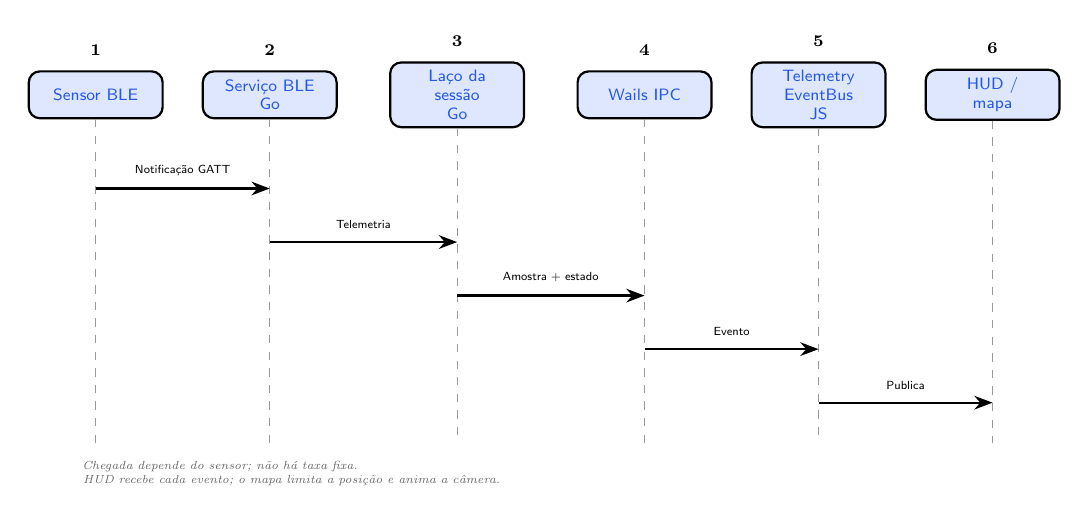
\begin{tikzpicture}[
    scale=0.85, every node/.style={transform shape},
    >=Stealth,
    actor/.style={rectangle, draw, rounded corners, minimum width=2.0cm,
      minimum height=0.7cm, align=center, font=\scriptsize\sffamily,
      fill=blueargus!15, text=blueargus!90!black, thick},
    edge node/.style={above, yshift=2pt, align=center, font=\tiny\sffamily},
    note/.style={font=\scriptsize\sffamily, align=center},
]

    % Lifelines
    \node[actor] (sensor) at (0,0) {Sensor BLE};
    \node[actor] (ble) at (2.6,0) {Serviço BLE\\Go};
    \node[actor] (sim) at (5.4,0) {Laço da\\sessão\\Go};
    \node[actor] (wails) at (8.2,0) {Wails IPC};
    \node[actor] (teb) at (10.8,0) {Telemetry\\EventBus\\JS};
    \node[actor] (canvas) at (13.4,0) {HUD /\\mapa};

    % Linhas tracejadas verticais
    \foreach \p in {sensor,ble,sim,wails,teb,canvas}
        \draw[dashed, black!40] (\p.south) -- (\p.south |- 0,-5.2);

    % Setas horizontais
    \draw[->, thick] (0,-1.4) -- node[edge node] {Notificação GATT}
        (2.6,-1.4);
    \draw[->, thick] (2.6,-2.2) -- node[edge node] {Telemetria}
        (5.4,-2.2);
    \draw[->, thick] (5.4,-3.0) -- node[edge node] {Amostra + estado}
        (8.2,-3.0);
    \draw[->, thick] (8.2,-3.8) -- node[edge node] {Evento}
        (10.8,-3.8);
    \draw[->, thick] (10.8,-4.6) -- node[edge node] {Publica}
        (13.4,-4.6);

    % Números sequenciais
    \node[note, font=\scriptsize\bfseries, above=3pt] at (sensor.north) {1};
    \node[note, font=\scriptsize\bfseries, above=3pt] at (ble.north) {2};
    \node[note, font=\scriptsize\bfseries, above=3pt] at (sim.north) {3};
    \node[note, font=\scriptsize\bfseries, above=3pt] at (wails.north) {4};
    \node[note, font=\scriptsize\bfseries, above=3pt] at (teb.north) {5};
    \node[note, font=\scriptsize\bfseries, above=3pt] at (canvas.north) {6};

    % Notas de comportamento
    \node[note, font=\tiny\itshape, text=black!60, anchor=north west,
        align=left, text width=12.4cm] at (-0.3,-5.35)
        {Chegada depende do sensor; não há taxa fixa.\\
         HUD recebe cada evento; o mapa limita a posição e anima a câmera.};

\end{tikzpicture}

\end{figure}

\section{Persistência e modelo de dados}
\label{sec:persistencia}

A persistência local é implementada sobre SQLite, acessado por meio do ORM
GORM \cite{gorm2024}. A aplicação mantém bancos de dados dedicados para o
histórico de atividades, os recordes de potência (curva MMP), o sistema de
gamificação e as classificações de eventos. As principais entidades do domínio
(\code{internal/domain}) são:

\begin{itemize}
    \item \code{UserProfile}: dados do atleta (nome, peso, FTP, frequências
        cardíacas, nível, XP, configurações e credenciais de integrações);
    \item \code{Activity}: sessão de treino concluída, com distância, elevação,
        métricas fisiológicas (NP, TSS, TRIMP, IF, desvio cardiovascular) e
        status de sincronização;
    \item \code{BikeComponent} e \code{ComponentReplacement}: componentes da
        bicicleta e seu histórico de substituições para o controle de desgaste;
    \item \code{EventRecord} e \code{SyncQueue}: classificações de eventos e a
        fila assíncrona de \textit{upload} para serviços externos;
    \item \code{AIConversation}: histórico de conversas do assistente de IA.
\end{itemize}

O acesso a essas entidades é orquestrado pela fachada
\code{StorageFacade}, que oferece uma interface limpa aos controladores Wails e
encapsula as transações entre os repositórios.

\section{Arquitetura móvel}
\label{sec:arquitetura-mobile}

No contexto móvel, o Capacitor encapsula a aplicação web e a comunicação com o
hardware é realizada pelo plugin \code{@capacitor-community/bluetooth-le}
\cite{capacitorble2024}, que expõe a antena BLE do dispositivo. Nessa
configuração, o motor de simulação física é executado em JavaScript
(\code{frontend/src/modules/CapacitorBluetoothService.js} e o motor portado),
permitindo o funcionamento autônomo do simulador em um smartphone sem o
\textit{backend} Go. A interface foi adaptada para operar em modo
\textit{landscape} (paisagem), priorizando a visibilidade do mapa 3D, como
ilustrado na Figura~\ref{fig:screenshot-mobile}.

\begin{figure}[htbp]
    \centering
    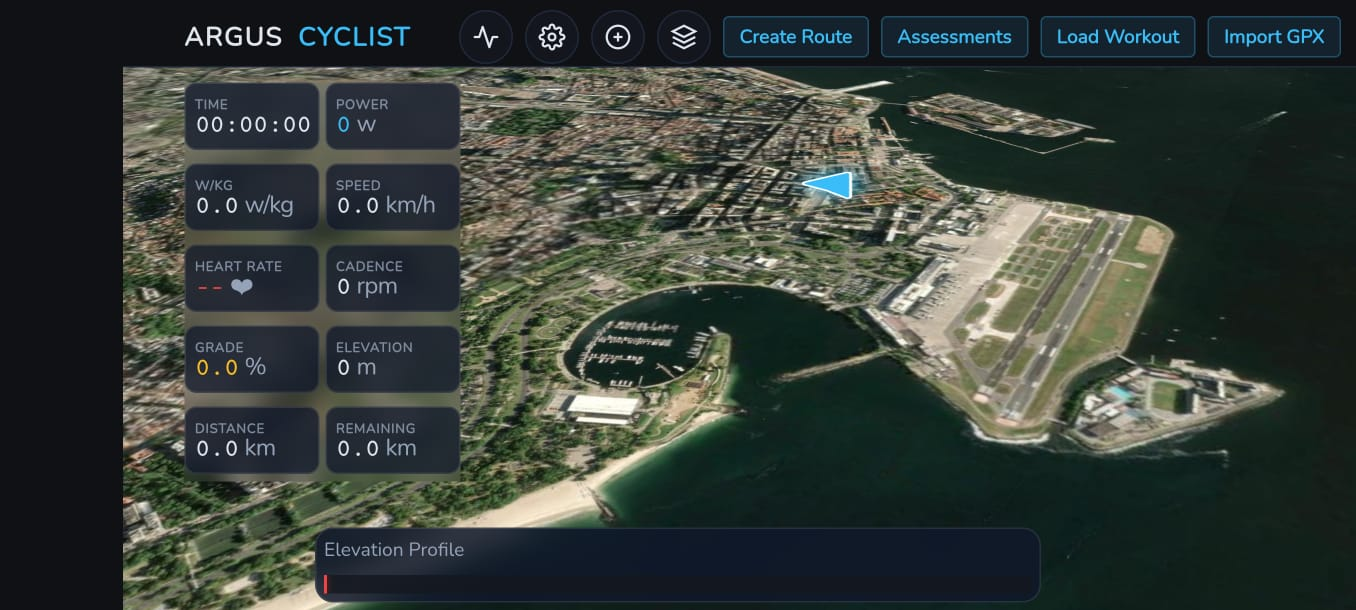
\includegraphics[width=0.85\textwidth]{figuras/screenshot-10-mobile}
    \caption{Aplicativo Android: HUD de simulação em modo \textit{landscape}}
    \label{fig:screenshot-mobile}
    \small Fonte: autoria própria.
\end{figure}

\section{Mapa mental do ecossistema}
\label{sec:diagrama-mapamental}

A Figura~\ref{fig:mapamental} apresenta o mapa mental do ecossistema \argus{},
organizando as principais funcionalidades e suas inter-relações.

\begin{figure}[htbp]
    \centering
    \caption{Mapa mental do ecossistema \argus{}}
    \label{fig:mapamental}
    % =====================================================================
%  DIAGRAMA 3 — MAPA MENTAL DO ECOSSISTEMA ARGUS CYCLIST
%  Fonte: autoria própria.
% =====================================================================
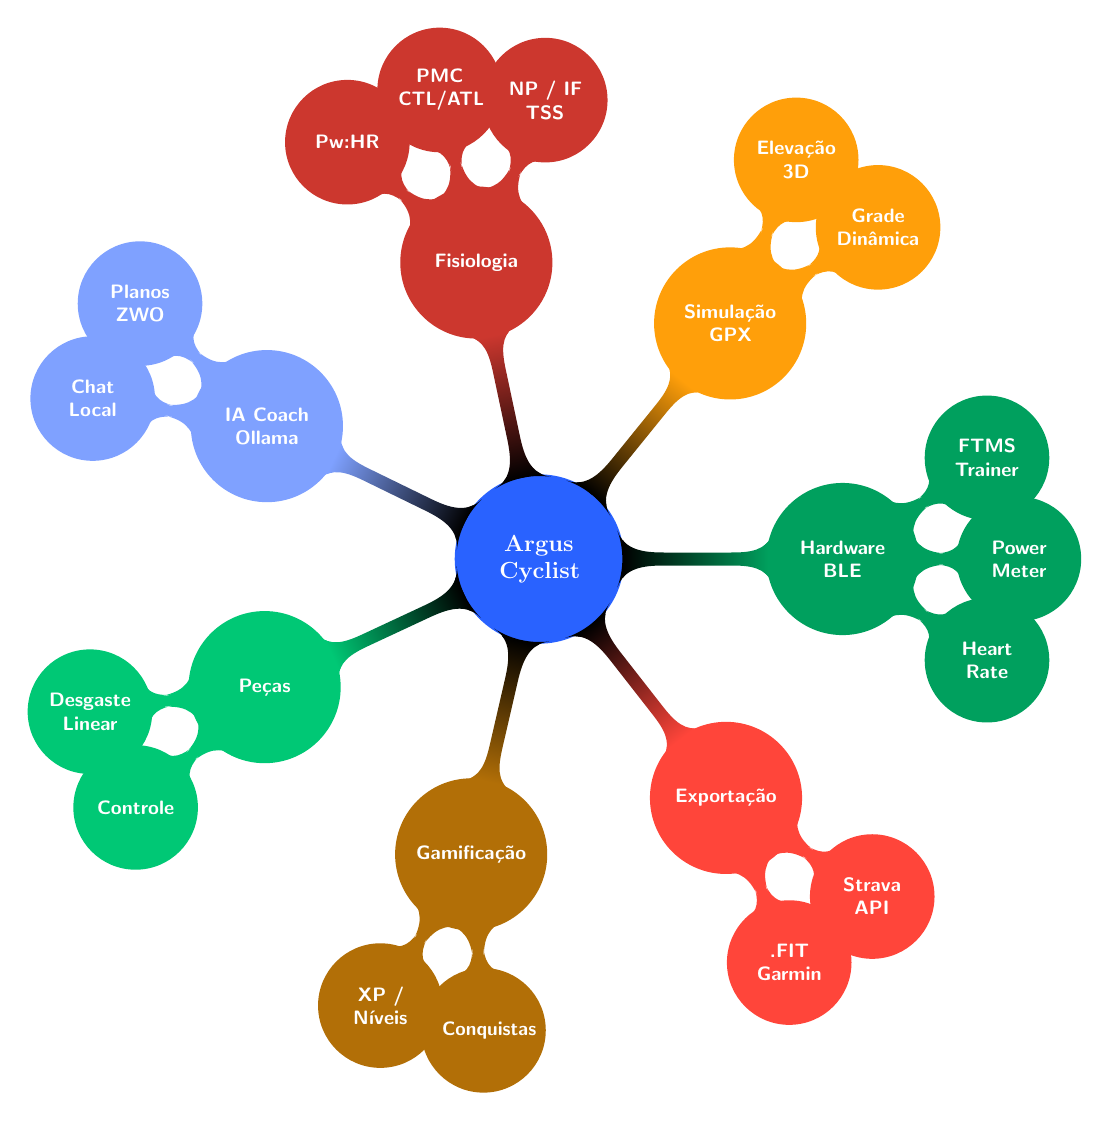
\begin{tikzpicture}[
    scale=0.7,
    transform shape,
    mindmap,
    every node/.style={concept, text=white, font=\sffamily\bfseries},
    root concept/.style={
      concept color=blueargus,
      minimum size=3.0cm,
      font=\large\bfseries,
      text width=2.8cm,
      align=center
    },
    level 1 concept/.append style={
      level distance=5.5cm,
      minimum size=2.7cm,
      font=\normalsize\bfseries,
      text width=2.0cm,
      align=center
    },
    level 2 concept/.append style={
      level distance=3.2cm,
      minimum size=2.2cm,
      font=\footnotesize\bfseries,
      text width=1.5cm,
      align=center
    },
]

      \node[root concept] {Argus\\Cyclist}
          % 1. Hardware BLE
          child[grow=0, concept color=greenargus!80!black] { node {Hardware\\BLE}
              child[grow=-35] { node {Heart\\Rate}}
              child[grow=0]   { node {Power\\Meter}}
              child[grow=35]  { node {FTMS\\Trainer}}
          }
          % 2. Simulação GPX
          child[grow=51.4, concept color=orangeargus] { node {Simulação\\GPX}
              child[grow=33.9] { node {Grade\\Dinâmica}}
              child[grow=68.9] { node {Elevação\\3D}}
          }
          % 3. Fisiologia
          child[grow=102.8, concept color=redargus!80!black] { node {Fisiologia}
              child[grow=67.8]  { node {NP / IF\\TSS}}
              child[grow=102.8] { node {PMC\\CTL/ATL}}
              child[grow=137.8] { node {Pw:HR}}
          }
          % 4. IA Coach Ollama
          child[grow=154.2, concept color=blueargus!60!white] { node {IA Coach\\Ollama}
              child[grow=136.7] { node {Planos\\ZWO}}
              child[grow=171.7] { node {Chat\\Local}}
          }
          % 5. Peças
          child[grow=205.7, concept color=greenargus] { node {Peças}
              child[grow=188.2] { node {Desgaste\\Linear}}
              child[grow=223.2] { node {Controle}}
          }
          % 6. Gamificação
          child[grow=257.1, concept color=orangeargus!70!black] { node {Gamificação}
              child[grow=239.6] { node {XP / Níveis}}
              child[grow=274.6] { node {Conquistas}}
          }
          % 7. Exportação
          child[grow=308.5, concept color=redargus] { node {Exportação}
              child[grow=291] { node {.FIT\\Garmin}}
              child[grow=326] { node {Strava\\API}}
          };
\end{tikzpicture}

\end{figure}

% =====================================================================
%  CAPÍTULO 5 — IMPLEMENTAÇÃO
% =====================================================================

\chapter{IMPLEMENTAÇÃO}
\label{cap:implementacao}

Este capítulo detalha a implementação do \argus{}, descrevendo a organização do
código-fonte, os principais módulos do \textit{backend} em Go e do
\textit{frontend} em JavaScript, as funcionalidades do sistema e os requisitos
atendidos.

\section{Visão geral do código}
\label{sec:visao-geral-codigo}

O repositório do projeto é organizado em três grandes áreas:

\begin{itemize}
    \item \code{app.go} e \code{gamification.go}: camada de aplicação
        exposta ao \textit{frontend} pelos \textit{bindings} Wails;
    \item \code{internal/}: núcleo do sistema, subdividido em \code{domain}
        (entidades e interfaces), \code{usecase} (fachadas), \code{service}
        (\code{ble}, \code{sim}, \code{gpx}, \code{fit}, \code{strava},
        \code{ai}, \code{workout}, \code{intervals}) e \code{repository}
        (persistência SQLite);
    \item \code{frontend/src/}: interface de usuário em JavaScript, com os
        módulos de controle (\code{modules/}), estilos (\code{styles/}) e
        componentes (\code{components/}).
\end{itemize}

Essa separação reflete a \textit{Clean Architecture} descrita no
Capítulo~\ref{cap:arquitetura} e viabiliza o desenvolvimento colaborativo e a
manutenibilidade do sistema.

\section{\textit{Backend} em Go}
\label{sec:backend}

\subsection{Módulo de conectividade BLE}
\label{sec:implementacao-ble}

O módulo \code{internal/service/ble} abstrai a comunicação com os sensores por
meio da biblioteca TinyGo Bluetooth \cite{tinygo2024}. Ele implementa o
escaneamento de dispositivos, a validação dos serviços GATT e a assinatura de
notificações para frequência cardíaca (\texttt{0x180D}), potência
(\texttt{0x1818}) e controle de rolos via FTMS (\texttt{0x1826}) e FE-C. A
comunicação é realizada por \textit{goroutines} concorrentes, de modo que a
recepção de telemetria não bloqueia a interface.

O módulo também disponibiliza um \textit{virtual trainer}, que simula o
comportamento de um rolo inteligente sem hardware físico, e \textit{mocks} para
viabilizar o desenvolvimento e os testes automatizados. Uma lista de dispositivos
BLE escaneados é exposta ao usuário por meio da interface de seleção explícita de
dispositivos.

\subsection{Motor de simulação física}
\label{sec:implementacao-sim}

O motor físico (\code{internal/service/sim}) implementa a equação de Martin
(Equação~\ref{eq:martin}) resolvida numericamente pelo método da bisseção, como
descrito na Seção~\ref{sec:equacao-martin}. A partir da potência instantânea
do atleta e do gradiente da rota, o motor calcula a velocidade virtual, que é
convertida em resistência mecânica enviada ao rolo em modo de simulação de
inclinação ou em potência alvo no modo ERG. O mesmo motor, portado para
JavaScript, é utilizado no aplicativo Android sem a necessidade do
\textit{backend} Go.

\subsection{Motor de métricas e exportação \texttt{.FIT}}
\label{sec:implementacao-fit}

O módulo \code{internal/service/fit} processa o vetor de \textit{samples} de
telemetria de \SI{1}{\hertz} e calcula as métricas fisiológicas: Potência
Normalizada (NP), Fator de Intensidade (IF), \textit{Training Stress Score}
(TSS), \textit{Training Impulse} (TRIMP) pela fórmula de Banister, tempo em
zonas de frequência cardíaca, recordes de potência (curva MMP) e o desvio
cardiovascular (Pw:HR). A biblioteca \code{muktihari/fit} \cite{fitgo2024} é
utilizada para serializar os dados no formato binário padrão Garmin/ANT+
\cite{garmin2024}, gerando arquivos compatíveis com Strava, Garmin Connect e
TrainingPeaks.

\subsection{Integração com serviços externos}
\label{sec:implementacao-externos}

A integração com o Strava (\code{internal/service/strava}) implementa o fluxo
OAuth 2.0 com \textit{refresh token} automático, utilizando um servidor HTTP
local para o \textit{callback} de autenticação. O \textit{upload} de atividades
é assíncrono e resiliente: falhas de rede são registradas em uma fila de
sincronização (\code{SyncQueue}) persistida no SQLite, com novas tentativas
programadas. A integração com o Intervals.icu
(\code{internal/service/intervals}) segue o mesmo padrão, ampliando a
interoperabilidade de dados do sistema.

\subsection{Assistente de treino com IA local}
\label{sec:implementacao-ai}

O assistente de IA (\code{internal/service/ai}) comunica-se com uma instância
do Ollama \cite{ollama2024} executada no dispositivo do usuário. O sistema
permite selecionar o modelo (por padrão, \texttt{qwen2.5:3b}), mantém o
histórico de conversas por perfil (\code{AIConversation}) e enriquece o
\textit{prompt} do sistema com os dados do atleta (FTP, nível, metas e
histórico recente de treinos). A partir da conversa, o assistente gera planos
de treino estruturados que são serializados no formato ZWO
(\code{saveWorkoutZWO}) e podem ser carregados diretamente no simulador em modo
ERG com um único clique.

\section{\textit{Frontend}}
\label{sec:frontend}

\subsection{Arquitetura e barramento de eventos}
\label{sec:frontend-eventbus}

O \textit{frontend} é implementado em JavaScript puro com Vite. O
\code{TelemetryEventBus} (em \code{frontend/src/modules/TelemetryEventBus.js})
desacopla a recepção de telemetria da renderização: os dados chegam do
\textit{backend} via \textit{bindings} Wails (ou do serviço BLE nativo do
Capacitor no Android) e são distribuídos aos assinantes (HUD, gráficos e
mapa) sem provocar \textit{reflows} globais, garantindo renderização fluida
a 60~fps.

\subsection{Mapa 3D e HUD}
\label{sec:frontend-mapa}

A renderização geográfica é realizada pelo MapLibre GL JS \cite{maplibre2024}
com terreno topográfico (Terrain-RGB), projeção globo 3D e temas claro/escuro.
A rota percorrida é colorida dinamicamente conforme o gradiente (verde para
trechos planos e vermelho para subidas íngremes), com o ciclista interpolado a
60~fps. O HUD exibe potência, cadência, frequência cardíaca, velocidade,
distância, elevação, zonas de potência e a barra de XP, com variações
especializadas para o modo Estúdio e para os modos de evento.

\subsection{Módulos de funcionalidades}
\label{sec:frontend-modulos}

O \textit{frontend} organiza as funcionalidades em módulos dedicados,
incluindo \code{MapController} (mapa e rota), \code{WorkoutController}
(treinos estruturados), \code{ChallengeController} (desafios e eventos),
\code{SummaryController} (resumo pós-treino), \code{AIChatController}
(assistente de IA), \code{FullscreenHUDController} (HUD em tela cheia),
\code{CapacitorBluetoothService} (BLE no Android) e \code{UIManager}
(orquestração da interface).

\section{Funcionalidades do sistema}
\label{sec:funcionalidades}

\subsection{Perfis de usuário e persistência local}
\label{sec:func-perfis}

O sistema suporta múltiplos perfis de atletas no mesmo dispositivo, cada um com
dados, nível, XP, FTP, peso e histórico de atividades isolados. A persistência
é 100\% local e \textit{offline-first}, com bancos SQLite dedicados para
atividades, recordes de potência, gamificação e eventos.

\subsection{Simulação e conectividade}
\label{sec:func-simulacao}

O \argus{} conecta-se a rolos inteligentes (FTMS e FE-C), medidores de potência
e cintas de frequência cardíaca, além de oferecer o \textit{virtual trainer}.
A resistência do rolo é controlada dinamicamente conforme o gradiente da rota,
o peso do atleta e o modo selecionado (ERG ou simulação de inclinação). A
Figura~\ref{fig:screenshot-telemetry} ilustra a telemetria em tempo real durante
uma sessão.

\begin{figure}[htbp]
    \centering
    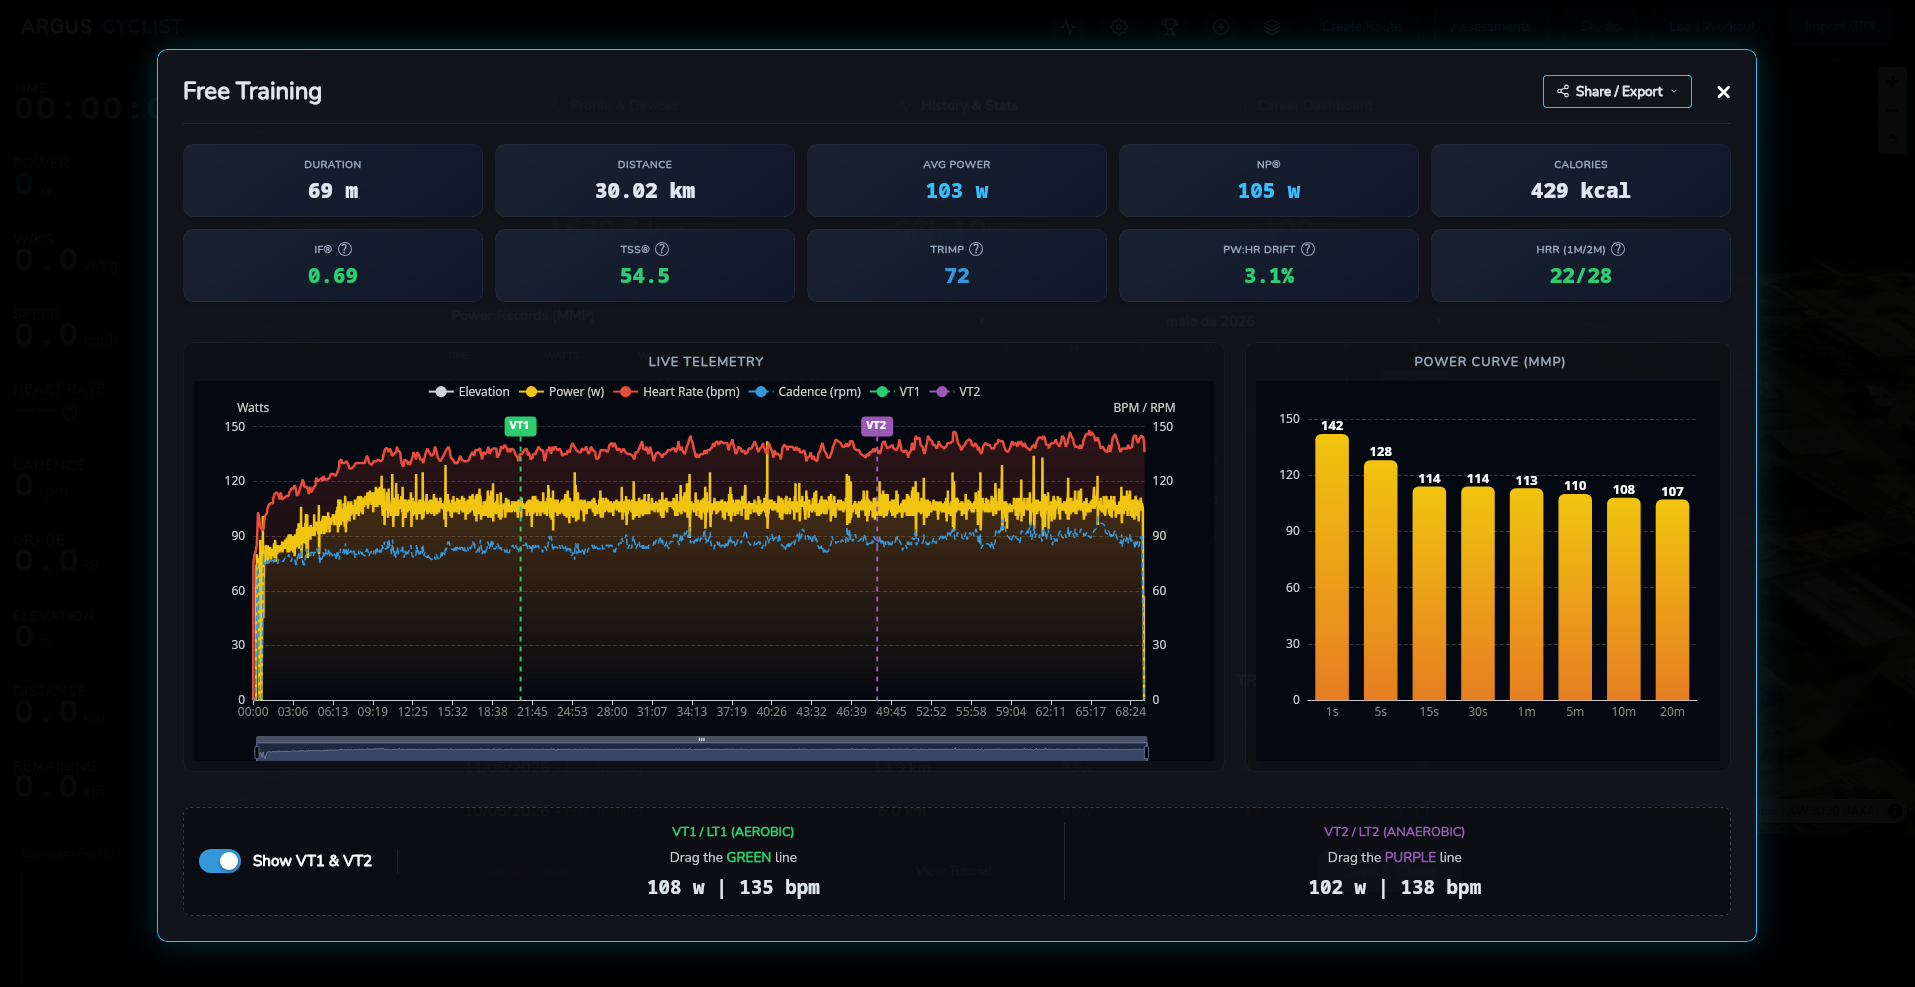
\includegraphics[width=0.85\textwidth]{figuras/screenshot-05-telemetry}
    \caption{Tela principal do simulador durante a sessão: telemetria em
    tempo real e mapa 3D}
    \label{fig:screenshot-telemetry}
    \small Fonte: autoria própria.
\end{figure}

\subsection{Treinos estruturados e avaliações de aptidão}
\label{sec:func-treinos}

Além do passeio livre, o sistema importa planos de treino ZWO e exibe os alvos
de potência em modo ERG, com ajuste de intensidade em tempo real. Avaliações
estruturadas de aptidão (\textit{Ramp Test} e teste de FTP) permitem estimar a
potência funcional limiar e calibrar as zonas de treino. A Figura~\ref{fig:screenshot-workout}
apresenta a execução de um treino estruturado.

\begin{figure}[htbp]
    \centering
    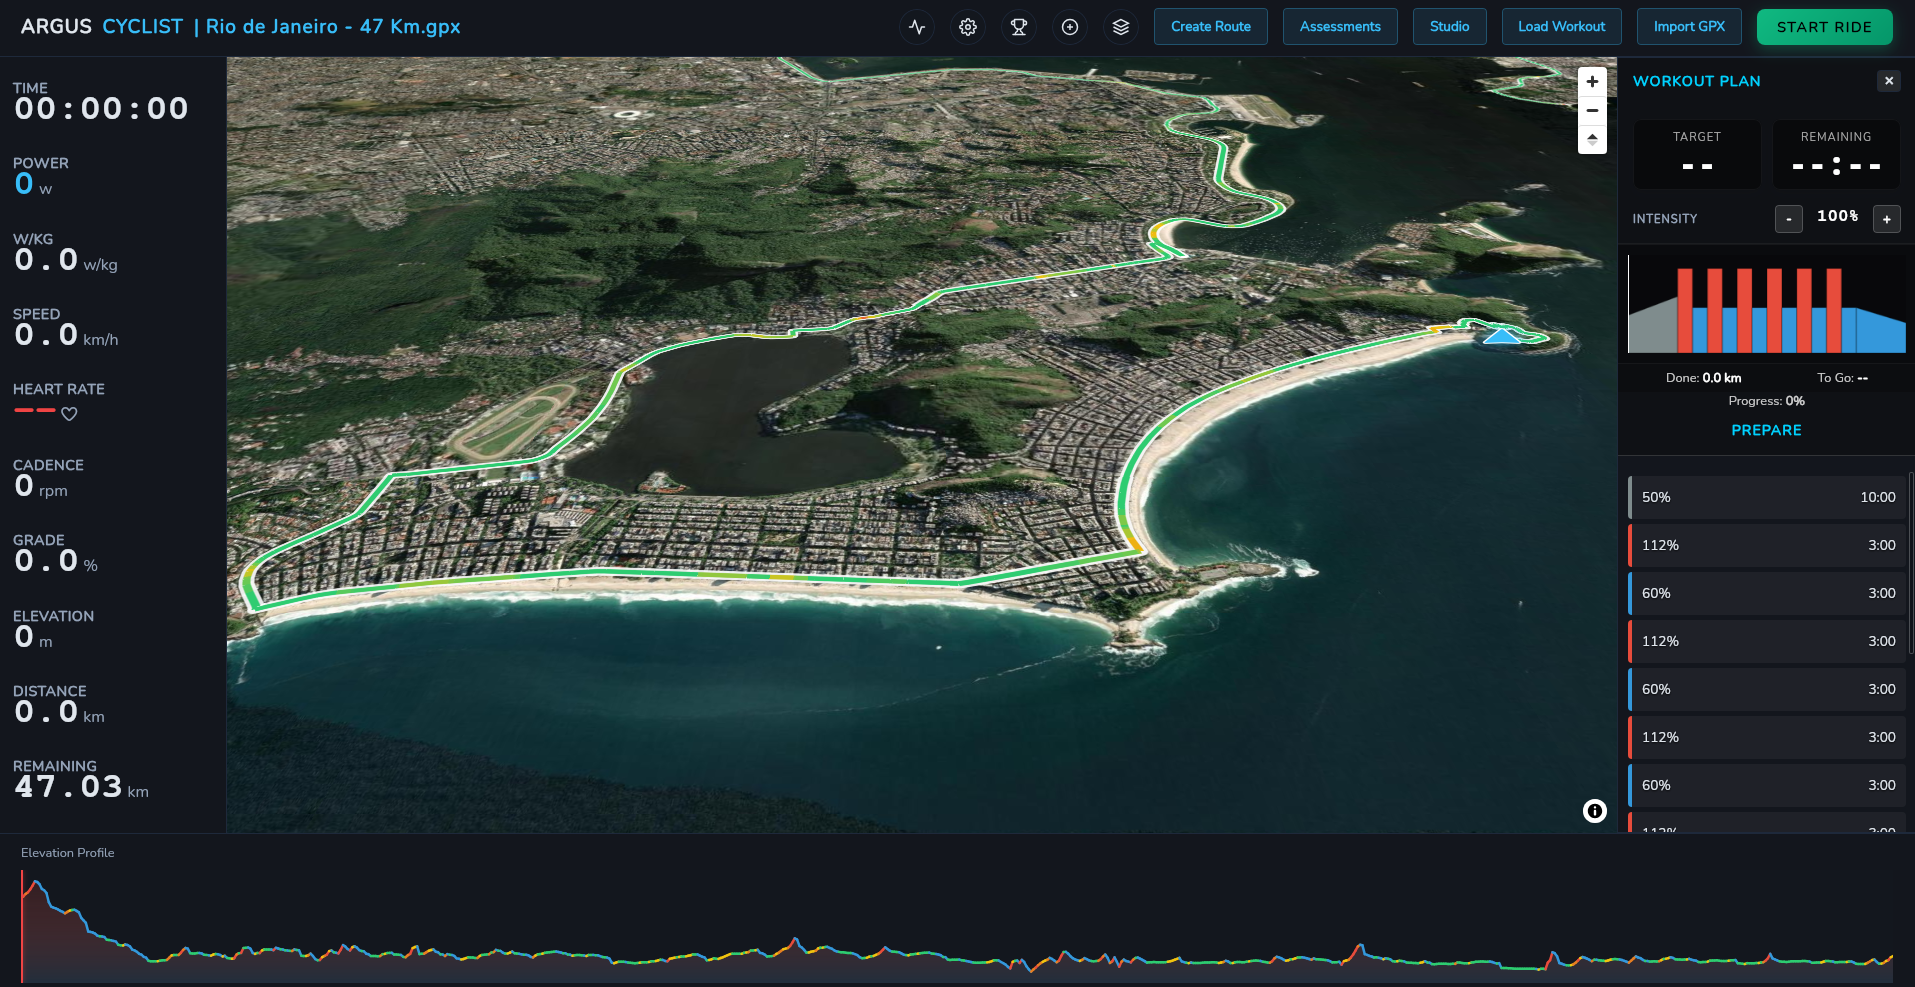
\includegraphics[width=0.85\textwidth]{figuras/screenshot-06-workout}
    \caption{Treino estruturado com alvo de potência em modo ERG}
    \label{fig:screenshot-workout}
    \small Fonte: autoria própria.
\end{figure}

\subsection{Modo Estúdio}
\label{sec:func-estudio}

O modo Estúdio (\textit{Studio Mode}) oferece um HUD dedicado à telemetria,
otimizado para aulas coletivas, com alvos de intervalo, zonas de potência e
cronômetros, sem o mapa 3D. A Figura~\ref{fig:screenshot-studio} ilustra esse
modo.

\begin{figure}[htbp]
    \centering
    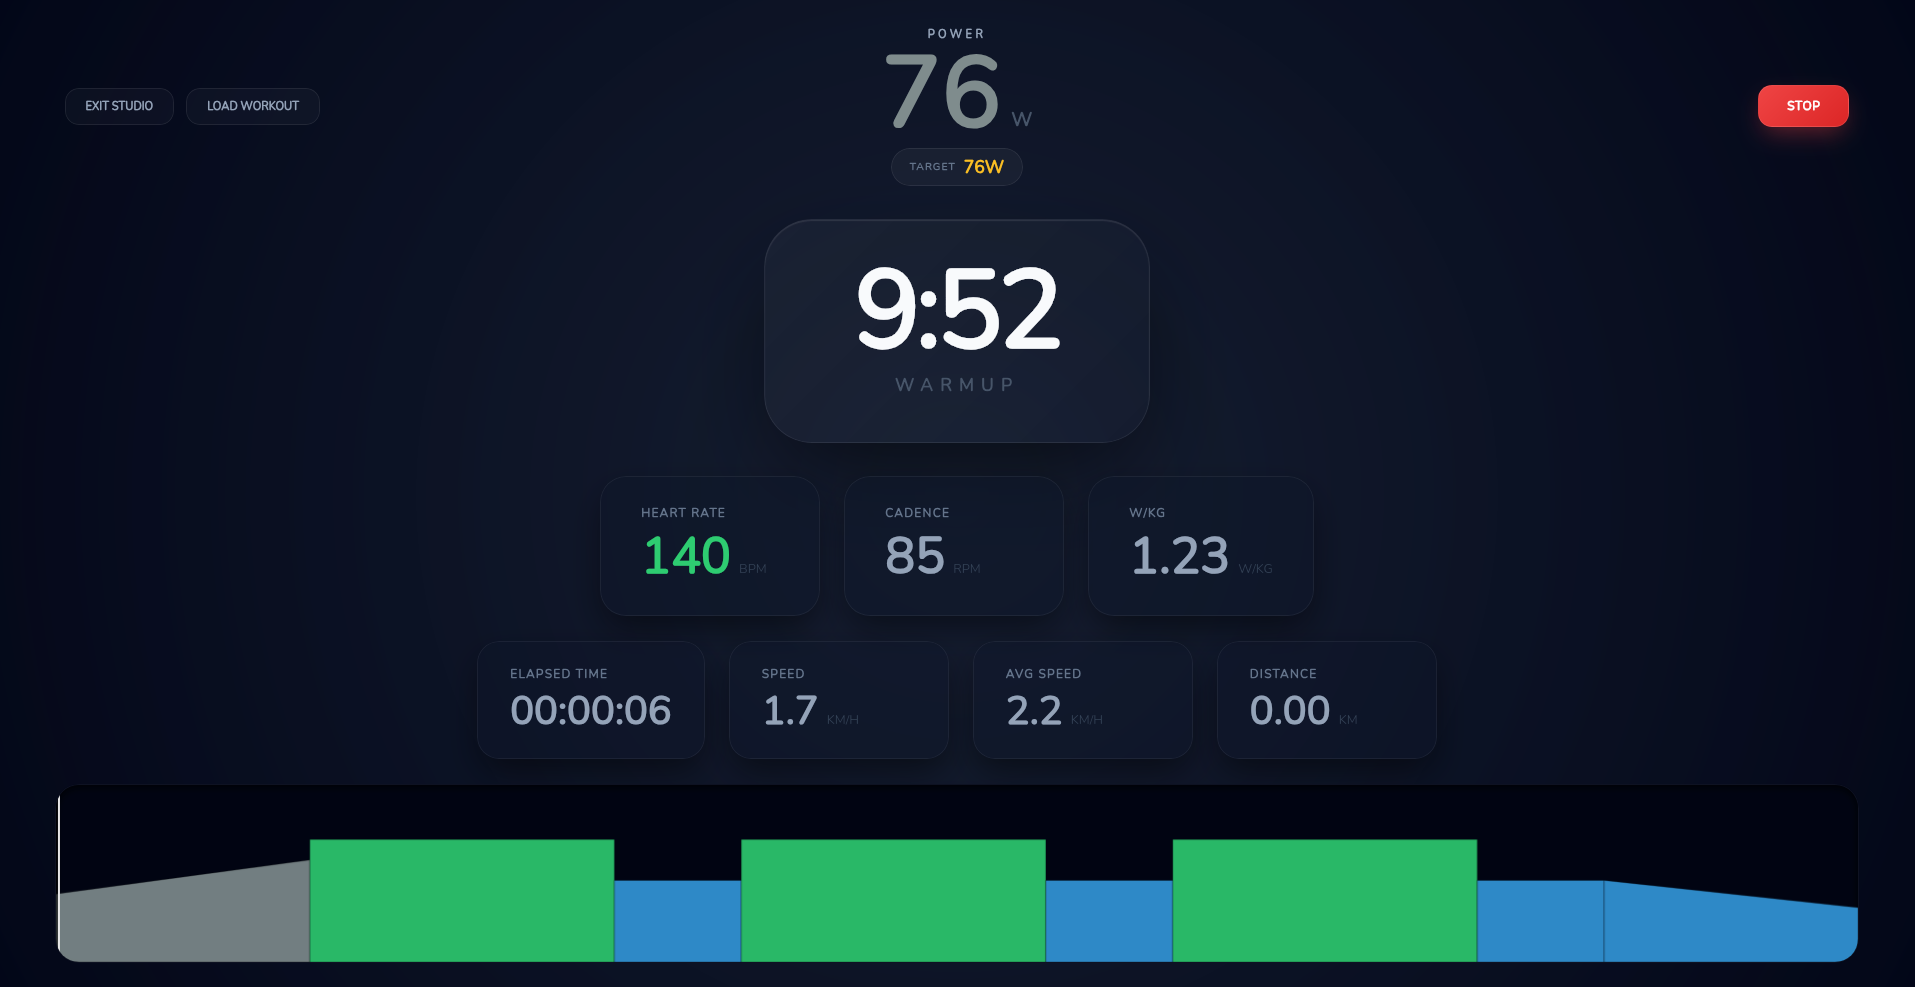
\includegraphics[width=0.85\textwidth]{figuras/screenshot-08-studio}
    \caption{Modo Estúdio: HUD de telemetria dedicado}
    \label{fig:screenshot-studio}
    \small Fonte: autoria própria.
\end{figure}

\subsection{Modo Evento}
\label{sec:func-evento}

O modo Evento (\textit{Event Mode}) permite a competição em desafios virtuais de
Sprint, KOM (\textit{King of the Mountain}) e Contrarrelógio (\textit{Time
Trial}), com regras de validação específicas e \textit{leaderboard} local
persistido em SQLite dedicado, incluindo filtros por gênero. A
Figura~\ref{fig:screenshot-event} apresenta a tela do modo evento.

\begin{figure}[htbp]
    \centering
    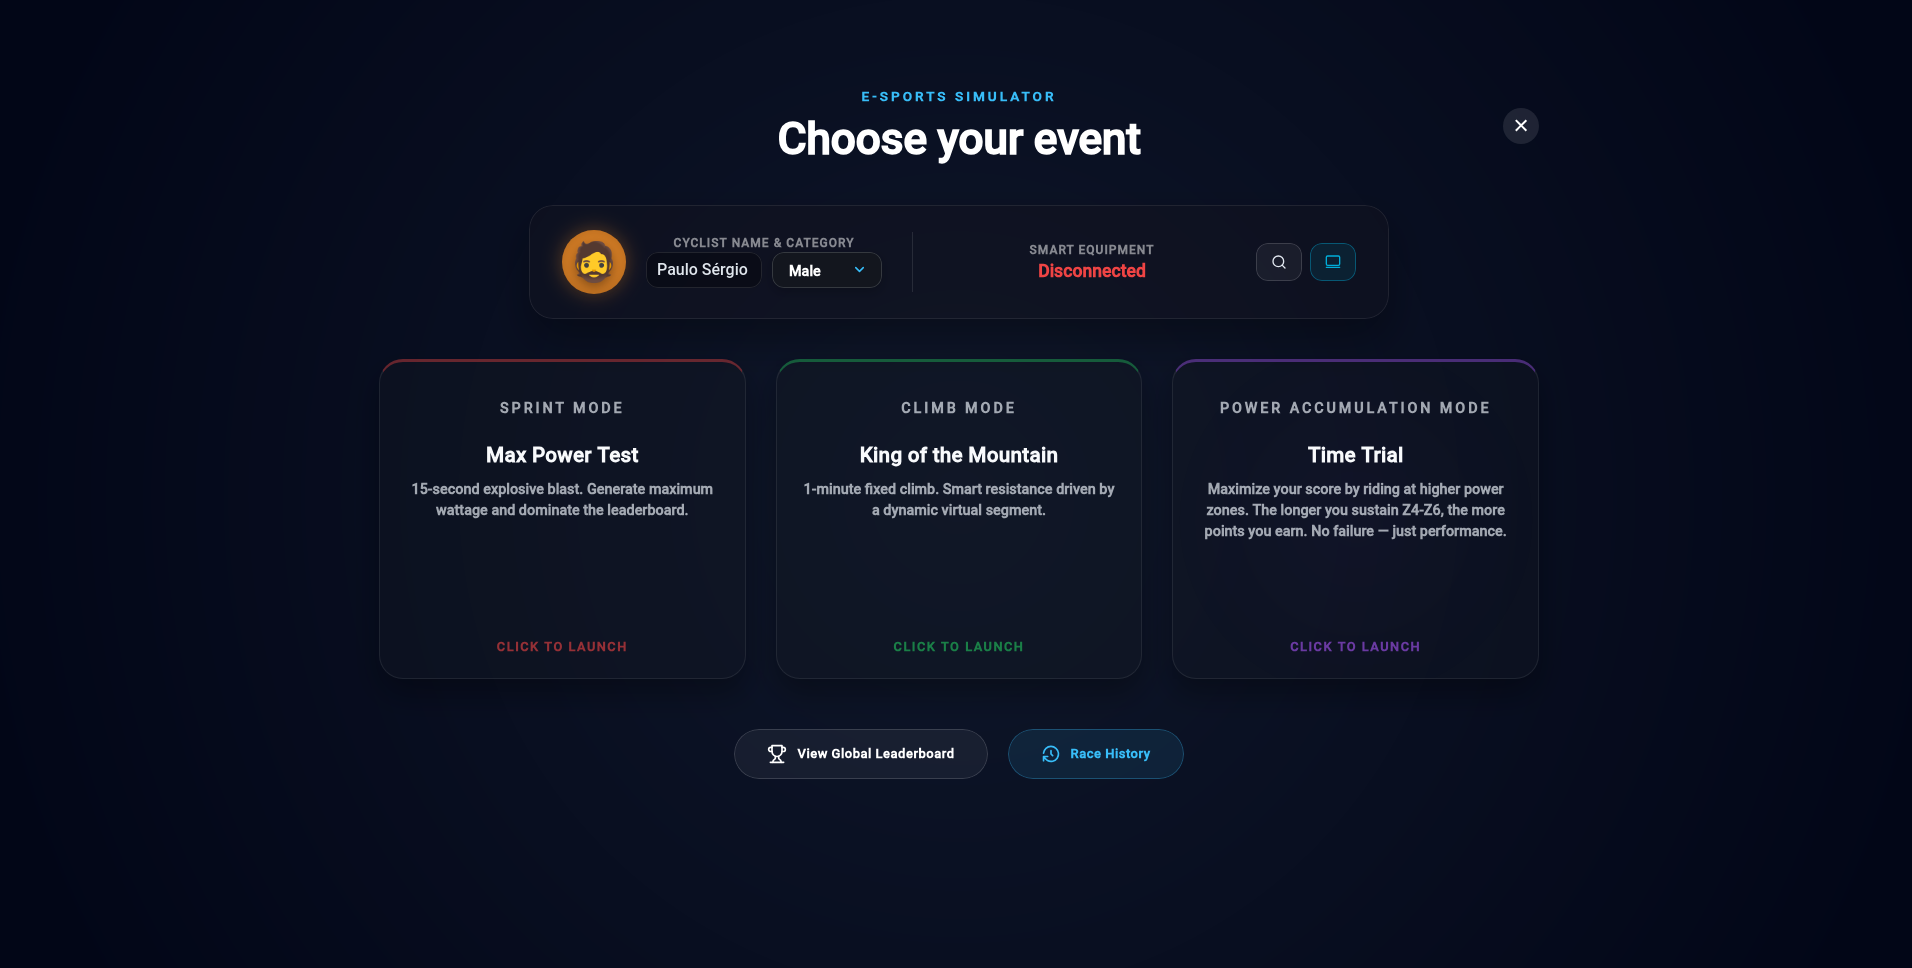
\includegraphics[width=0.85\textwidth]{figuras/screenshot-09-event}
    \caption{Modo Evento: desafio virtual com classificação local}
    \label{fig:screenshot-event}
    \small Fonte: autoria própria.
\end{figure}

\subsection{Gamificação}
\label{sec:func-gamificacao}

O sistema de gamificação (\code{gamification.go}) atribui XP passivamente
durante os treinos, com recompensas adicionais para subidas e longas
distâncias. Níveis, troféus, conquistas de consistência/recuperação/rotina e
metas personalizadas (\code{CustomGoal}) são persistidos por perfil e exibidos
na \textit{Trophy Room} (Figura~\ref{fig:screenshot-trophy}).

\begin{figure}[htbp]
    \centering
    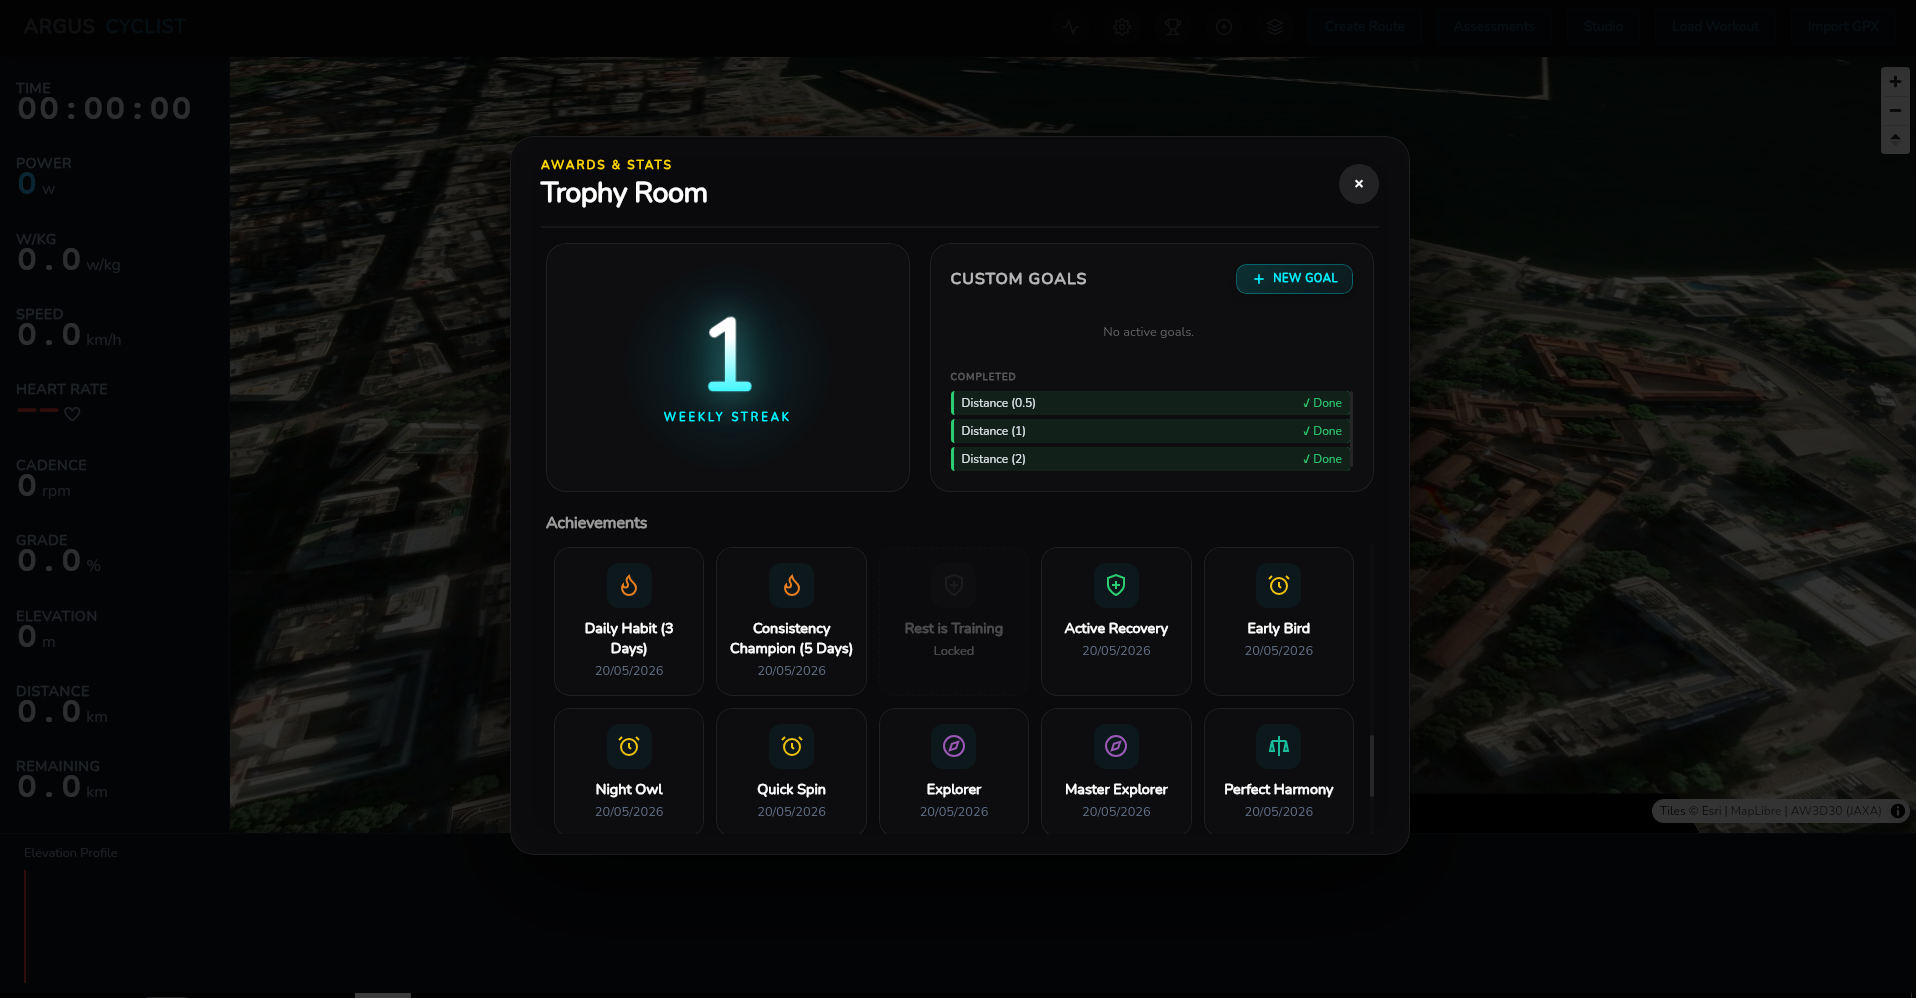
\includegraphics[width=0.85\textwidth]{figuras/screenshot-07-trophy}
    \caption{Trophy Room: troféus e conquistas do atleta}
    \label{fig:screenshot-trophy}
    \small Fonte: autoria própria.
\end{figure}

\subsection{Assistente de treino com IA}
\label{sec:func-ia}

O assistente de treino permite conversar em linguagem natural com um modelo de
linguagem local (Ollama), que considera o perfil do atleta e o histórico
recente para sugerir treinos e gerar planos ZWO carregáveis no simulador. As
conversas são persistidas por perfil e o modelo é selecionável pelo usuário.

\subsection{Rastreamento de desgaste de componentes}
\label{sec:func-componentes}

O módulo de componentes (\code{BikeComponent}) permite cadastrar peças da
bicicleta (corrente, cassete, coroas, etc.) com vida útil estimada em
quilômetros. Ao final de cada sessão, o desgaste é atualizado automaticamente
pela razão entre a distância acumulada e a vida útil, com indicadores visuais
codificados por cores (verde, amarelo e vermelho) e histórico de substituições
(\code{ComponentReplacement}) com auditoria temporal. A
Figura~\ref{fig:screenshot-desgaste} apresenta a tela de rastreamento de
componentes.

\begin{figure}[htbp]
    \centering
    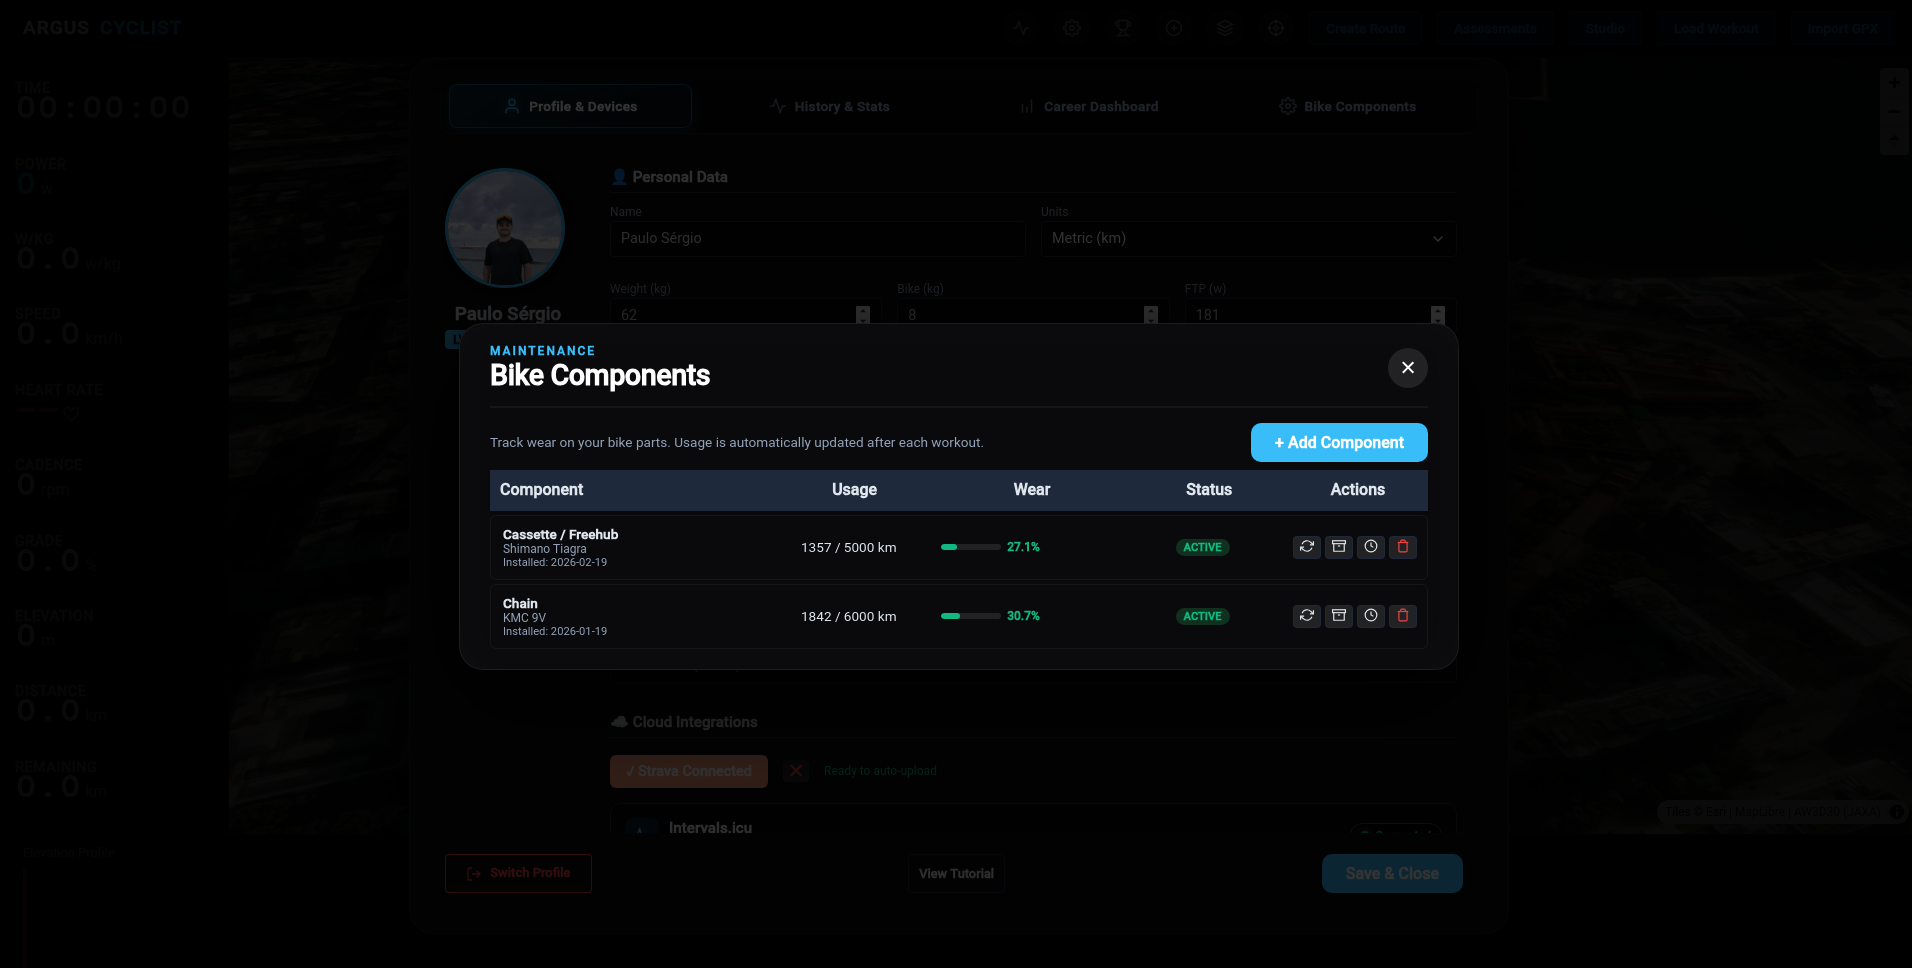
\includegraphics[width=0.85\textwidth]{figuras/screenshot-11-desgaste}
    \caption{Rastreamento de desgaste de componentes mecânicos}
    \label{fig:screenshot-desgaste}
    \small Fonte: autoria própria.
\end{figure}

\section{Requisitos funcionais e não funcionais}
\label{sec:requisitos}

A especificação de requisitos foi derivada da necessidade de estabilidade em
tempo real e de conformidade com os padrões de arquivos esportivos. As Tabelas
\ref{tab:rf} e \ref{tab:rnf} apresentam os requisitos funcionais e não
funcionais do sistema.

\begin{table}[h]
    \centering
    \caption{Requisitos funcionais do \argus{}}
    \label{tab:rf}
    \small
    \begin{tabular}{
        >{\raggedright\arraybackslash}p{4.2cm}
        >{\raggedright\arraybackslash}p{10.2cm}
    }
        \toprule
        \textbf{Identificador} & \textbf{Descrição} \\
        \midrule
        RF01 & Gestão de sensores BLE: escaneamento, pareamento e recepção de
        dados via perfis GATT de frequência cardíaca, potência e cadência. \\
        RF02 & Controle de equipamento (FTMS/FE-C): envio de comandos de
        resistência para rolos inteligentes em modo ERG ou simulação de
        inclinação. \\
        RF03 & Motor de simulação GPX: interpretação de rotas GPX e cálculo da
        velocidade virtual baseado no peso do atleta, potência e inclinação. \\
        RF04 & Registro de atividade (FIT SDK): geração de arquivos binários
        \texttt{.fit} com todos os \textit{samples} de telemetria da sessão. \\
        RF05 & Integração Strava: autenticação OAuth 2.0 e \textit{upload}
        automático de sessões finalizadas. \\
        RF06 & Persistência local: armazenamento de usuários, configurações,
        histórico de atividades e recordes em SQLite local. \\
        RF07 & Desafios e gamificação: desafios de segmentos (Sprints e KOM) e
        avaliações de capacidade (teste FTP) durante a simulação. \\
        RF08 & Assistente de IA local: geração de planos de treino ZWO
        personalizados via Ollama. \\
        RF09 & Controle de desgaste de componentes: cadastro e cálculo automático
        de desgaste de peças com histórico de substituições. \\
        RF10 & Integração Intervals.icu: \textit{upload} de atividades
        finalizadas. \\
        \bottomrule
    \end{tabular}
\end{table}

\begin{table}[h]
    \centering
    \caption{Requisitos não funcionais do \argus{}}
    \label{tab:rnf}
    \small
    \begin{tabular}{
        >{\raggedright\arraybackslash}p{4.2cm}
        >{\raggedright\arraybackslash}p{10.2cm}
    }
        \toprule
        \textbf{Identificador} & \textbf{Descrição} \\
        \midrule
        RNF01 & Latência de telemetria: o tempo entre a recepção do pacote BLE e
        a atualização na interface não deve exceder \SI{150}{\milli\second}. \\
        RNF02 & Portabilidade: a base de código deve ser compilável para Windows
        (Wails), Linux e Android (Capacitor) sem perda de funcionalidades. \\
        RNF03 & Estabilidade de conexão: rotinas de auto-reconexão para sensores
        que percam sinal durante a sessão. \\
        RNF04 & Eficiência de memória: o \textit{backend} em Go não deve exceder
        \SI{200}{\mega\byte} de \textit{footprint} durante a simulação ativa. \\
        RNF05 & Privacidade: processamento local de dados biométricos, com
        integrações externas apenas sob consentimento explícito do usuário. \\
        RNF06 & Licenciamento: distribuição sob licença GPLv3
        \cite{gpl2007}. \\
        \bottomrule
    \end{tabular}
\end{table}

% =====================================================================
%  CAPÍTULO 6 — RESULTADOS E VALIDAÇÃO
% =====================================================================

\chapter{RESULTADOS E VALIDAÇÃO}
\label{cap:resultados}

Este capítulo apresenta os resultados do desenvolvimento do \argus{}, a
estratégia de validação adotada e as evidências de que o software atende aos
requisitos funcionais e não funcionais definidos.

\section{Estratégia de validação}
\label{sec:estrategia-validacao}

A validação do software foi conduzida em três frentes complementares:

\begin{itemize}
    \item \textbf{Validação funcional}: execução das funcionalidades do sistema
        em cenários reais de uso, verificando a conformidade com os requisitos
        funcionais (Tabela~\ref{tab:rf});
    \item \textbf{Validação experimental}: testes com equipamentos reais de
        ciclismo (rolos inteligentes e medidores de potência), aferindo
        estabilidade de conexão e latência de telemetria;
    \item \textbf{Validação de conformidade}: submissão dos arquivos
        \texttt{.fit} gerados a plataformas de análise (Strava e Intervals.icu)
        para comprovar a exatidão estrutural e estatística dos dados.
\end{itemize}

\section{Validação funcional}
\label{sec:validacao-funcional}

As funcionalidades implementadas foram exercitadas em ambiente real, cobrindo o
ciclo completo de treinamento: conexão com sensores, execução de sessões
livres e estruturadas, modos de evento e estúdio, gamificação, geração de
arquivos \texttt{.fit} e integrações com o Strava e o Intervals.icu. Os testes
foram conduzidos manualmente pelo autor ao longo do desenvolvimento, percorrendo
todas as funcionalidades descritas no Capítulo~\ref{cap:implementacao} sem
registro formal em planilha ou relatório de testes. A Figura~\ref{fig:screenshot-career}
ilustra o \textit{dashboard} de carreira com o gráfico PMC, e a
Figura~\ref{fig:screenshot-history} apresenta o histórico de atividades com as
métricas calculadas.

\begin{figure}[htbp]
    \centering
    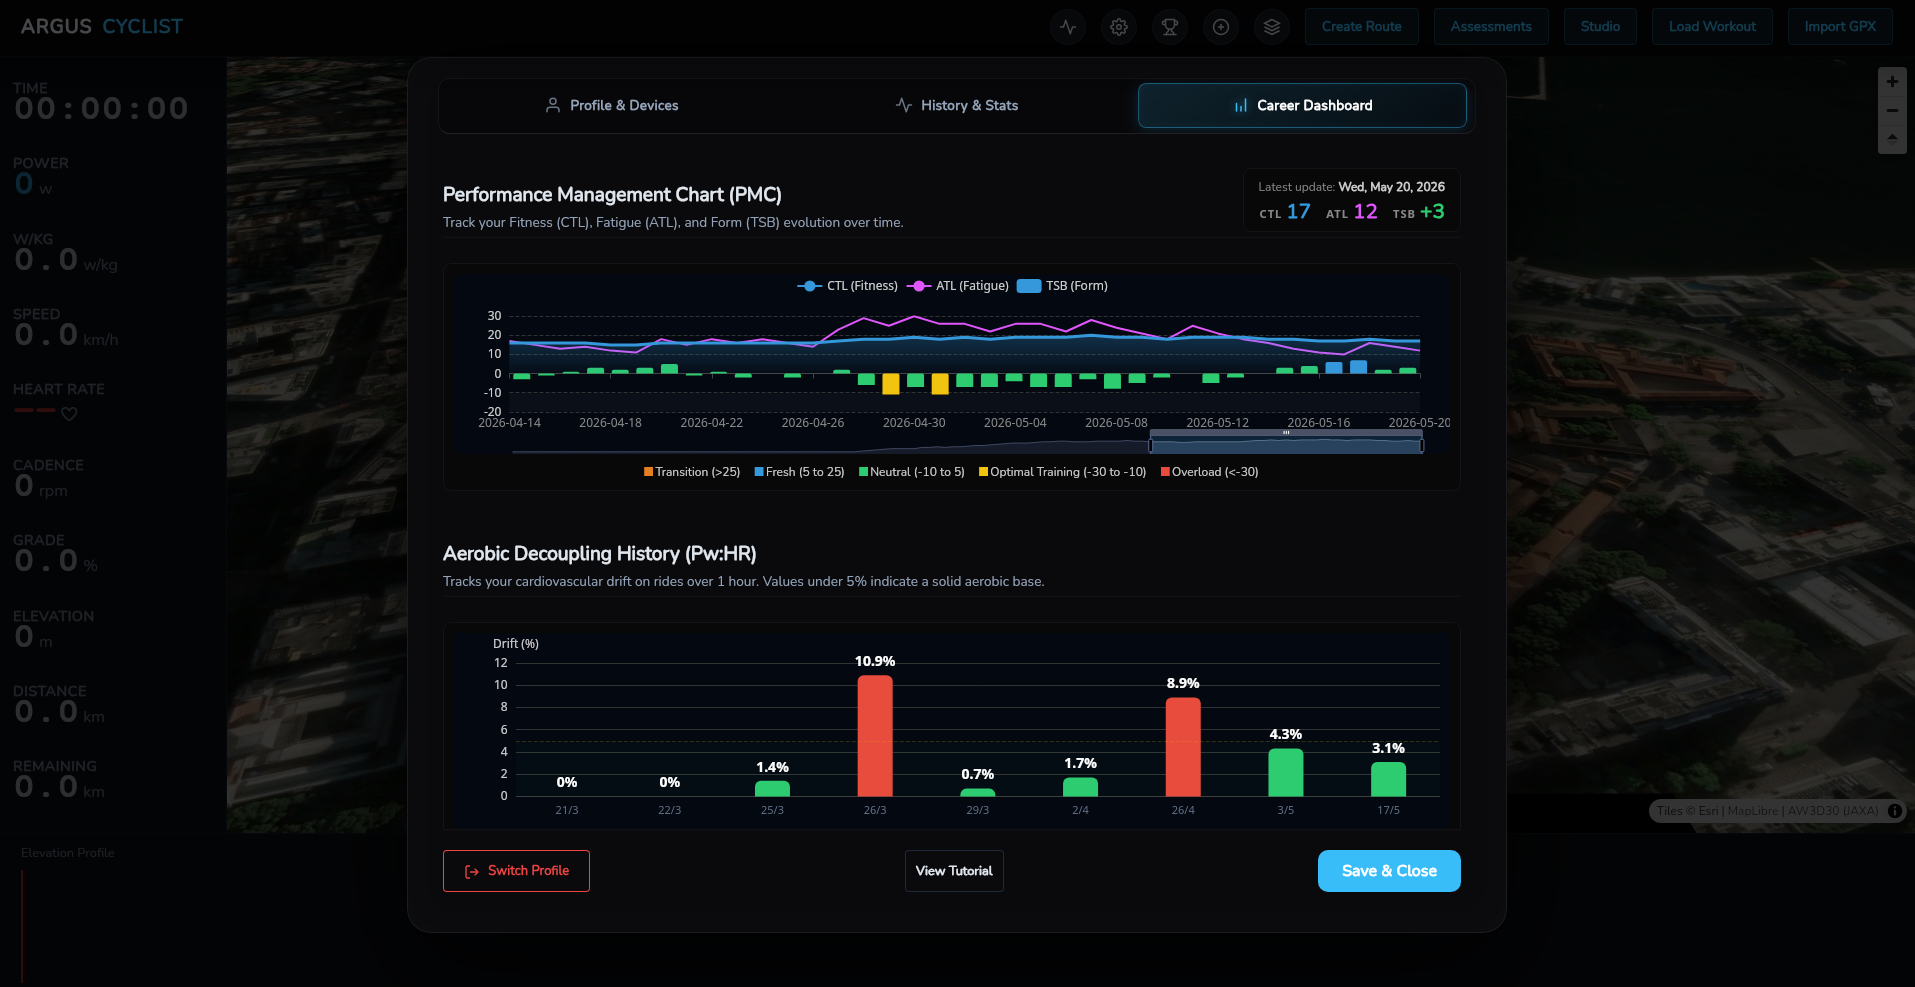
\includegraphics[width=0.85\textwidth]{figuras/screenshot-04-career}
    \caption{\textit{Dashboard} de carreira: PMC (CTL/ATL/TSB) e desvio cardiovascular}
    \label{fig:screenshot-career}
    \small Fonte: autoria própria.
\end{figure}

\begin{figure}[htbp]
    \centering
    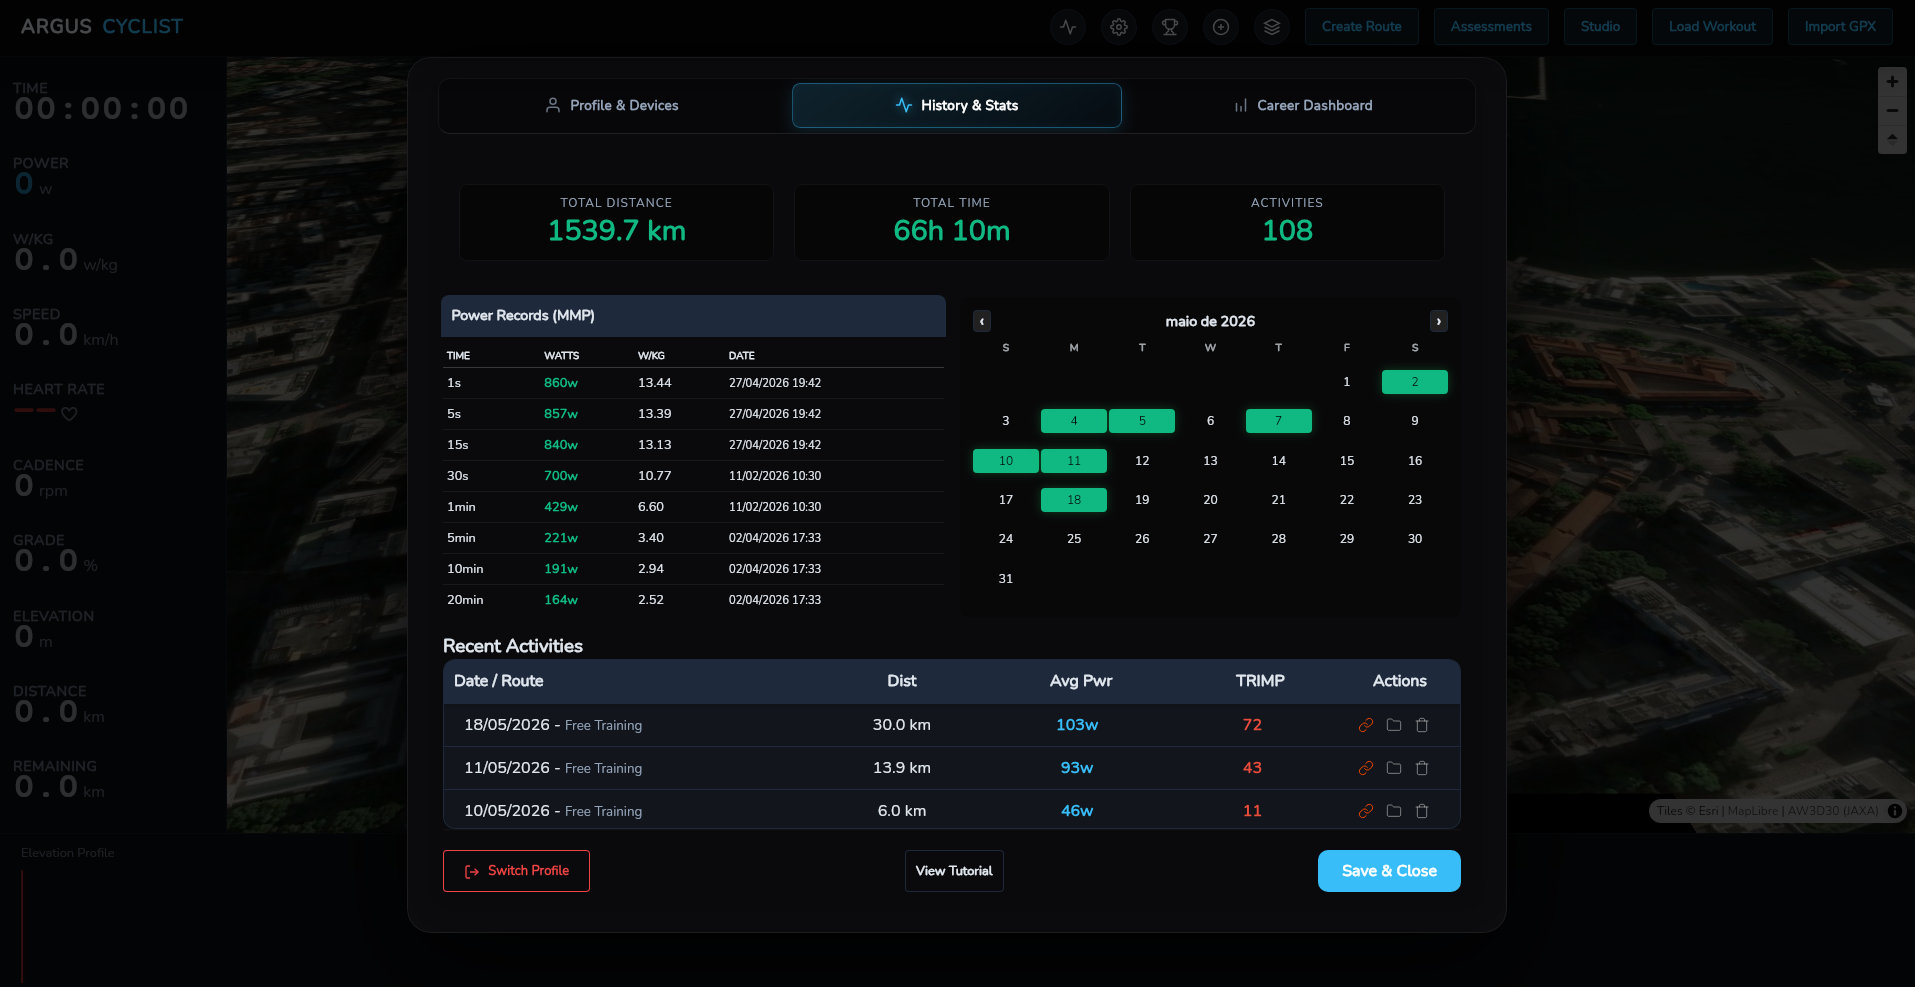
\includegraphics[width=0.85\textwidth]{figuras/screenshot-03-history}
    \caption{Histórico de atividades com métricas fisiológicas}
    \label{fig:screenshot-history}
    \small Fonte: autoria própria.
\end{figure}

\section{Validação experimental}
\label{sec:validacao-experimental}

A validação experimental foi realizada com equipamentos reais de ciclismo. O
\argus{} foi utilizado com o rolo inteligente (\textit{smart trainer}) ThinkRider
X2 MAX, a cinta de frequência cardíaca Cyplus H1 e um sensor de velocidade
(\textit{bike speed}). A comunicação também foi exercitada com a bicicleta
ergométrica Spinning SB 2000 Genis. Os testes foram conduzidos em três ambientes:
um notebook com Arch Linux, um PC com Windows 11 e um celular com Android. O
objetivo foi verificar a estabilidade das conexões BLE durante sessões contínuas
e a latência de telemetria entre a recepção do pacote e a atualização na
interface, comparando-a com o limite de \SI{150}{\milli\second} definido no
requisito RNF01.

\begin{table}[h]
    \centering
    \caption{Resultados da validação experimental}
    \label{tab:validacao}
    \small
    \begin{tabular}{
        >{\raggedright\arraybackslash}p{5.5cm}
        >{\centering\arraybackslash}p{2.6cm}
        >{\centering\arraybackslash}p{2.6cm}
        >{\centering\arraybackslash}p{3cm}
    }
        \toprule
        \textbf{Métrica} & \textbf{Alvo} & \textbf{Aferido} &
        \textbf{Conformidade} \\
        \midrule
        Latência de telemetria (sensor $\rightarrow$ tela) &
        $<$ \SI{150}{\milli\second} &
        $\sim$\SI{80}{\milli\second} &
        sim \\
        Estabilidade da conexão BLE (sessão contínua) &
        até 3~horas &
        3~horas sem desconexões &
        sim \\
        Consumo de memória do \textit{backend} (Go) &
        $<$ \SI{200}{\mega\byte} &
        $\sim$\SI{85}{\mega\byte} &
        sim \\
        \bottomrule
    \end{tabular}
\end{table}

A estabilidade da conexão BLE foi confirmada em sessões contínuas de até 3
horas de pedal, sem nenhuma desconexão do rolo inteligente ou da cinta de
frequência cardíaca. A latência de telemetria foi aferida em
$\sim$\SI{80}{\milli\second} (dentro do limite de \SI{150}{\milli\second}
definido no RNF01), e o consumo de memória do \textit{backend} foi de
$\sim$\SI{85}{\mega\byte} durante a simulação ativa (muito abaixo do limite
de \SI{200}{\mega\byte} do RNF04).

\section{Validação de conformidade dos dados (\texttt{.fit})}
\label{sec:validacao-conformidade}

Ao longo do desenvolvimento foram gerados mais de 200 arquivos \texttt{.fit}
no formato binário padrão Garmin/ANT+ \cite{garmin2024}. Todos foram exportados
para o Strava e o Intervals.icu (por meio da integração nativa de
\textit{upload}) e aceitos sem erros de importação, confirmando a
conformidade estrutural e estatística dos dados. Após a importação, as métricas
apresentadas por essas plataformas (distância, potência, elevação, frequência
cardíaca) conferiram com os valores registrados durante as sessões.

\section{Requisitos não funcionais}
\label{sec:rnf-atendidos}

A Tabela~\ref{tab:rnf} definiu os requisitos não funcionais do sistema. Todos
foram atendidos: a estabilidade de conexão (RNF03) foi confirmada em sessões
contínuas de até 3 horas sem desconexões; a portabilidade (RNF02) foi
exercitada com execução em Windows 11, Arch Linux e Android; a latência de
telemetria (RNF01) ficou em $\sim$\SI{80}{\milli\second}, inferior ao limite
de \SI{150}{\milli\second}; o consumo de memória (RNF04) foi de
$\sim$\SI{85}{\mega\byte}, abaixo do limite de \SI{200}{\mega\byte}; e o
processamento local e o licenciamento GPLv3 (RNF05 e RNF06) são garantidos
pela arquitetura e pela distribuição do código.

\section{Limitações e desafios}
\label{sec:limitacoes}

Durante o desenvolvimento, foram identificadas limitações e desafios que
orientam trabalhos futuros:

\begin{itemize}
    \item \textbf{Inferência da IA local}: a geração de planos de treino em
        dispositivos sem aceleração por GPU pode ser lenta, exigindo modelos
        quantizados e otimizações de \textit{prompt};
    \item \textbf{Validação com mais equipamentos}: a validação experimental
        concentrou-se em um conjunto específico de rolos e sensores, sendo
        desejável ampliar a cobertura de fabricantes e protocolos;
    \item \textbf{Disponibilidade de mapas offline}: a renderização do mapa 3D
        depende de \textit{tiles} obtidos da rede, havendo margem para caching
        local mais robusto em cenários totalmente \textit{offline};
    \item \textbf{Modo multiplayer}: o sistema é local e não contempla a
        interação social em tempo real entre atletas, uma funcionalidade
        central das plataformas comerciais.
\end{itemize}

% =====================================================================
%  CAPÍTULO 7 — CONCLUSÃO
% =====================================================================

\chapter{CONCLUSÃO}
\label{cap:conclusao}

Este trabalho apresentou o registro de software do \argus{}, um simulador
multiplataforma de ciclismo virtual de código aberto, e documentou a evolução
do projeto desde a versão inicial registrada junto ao INPI até a versão atual.
O desenvolvimento demonstrou a viabilidade técnica de uma plataforma de
ciclismo virtual gratuita, multiplataforma e orientada ao processamento local.

\section{Considerações finais}
\label{sec:consideracoes-finais}

O \argus{} diferencia-se por combinar simulação física em tempo real, análise
fisiológica avançada, integração com dispositivos BLE e recursos de
inteligência artificial executados localmente, preservando a privacidade dos
usuários e reduzindo dependências de infraestrutura em nuvem. Adicionalmente, o
sistema de rastreamento de desgaste de componentes oferece uma ferramenta
prática de manutenção preventiva, preenchendo uma lacuna não endereçada pelas
plataformas comerciais existentes.

A arquitetura em \textit{Clean Architecture}, com os padrões \textit{Facade} e
\textit{Repository}, demonstrou-se adequada para o domínio: permitiu a evolução
contínua do sistema --- como a adição do aplicativo Android, das integrações
com o Strava e o Intervals.icu e do assistente de IA --- sem comprometer a
estabilidade dos módulos existentes. A validação experimental com equipamentos
reais confirmou o atendimento a todos os requisitos funcionais e não
funcionais definidos.

Além da contribuição tecnológica, a proposta possui relevância social
significativa ao democratizar o acesso ao treinamento esportivo científico,
especialmente para atletas amadores e usuários com limitações financeiras ou
computacionais. Dessa forma, o \argus{} consolida-se como uma alternativa
inovadora às soluções proprietárias do mercado, unindo acessibilidade,
desempenho e liberdade tecnológica.

\section{Rastreabilidade de objetivos}
\label{sec:rastreabilidade}

A Tabela~\ref{tab:rastreabilidade} apresenta a relação entre os objetivos
específicos definidos no Capítulo~\ref{cap:introducao}, as implementações
realizadas e as evidências de validação.

\begin{table}[h]
    \centering
    \caption{Rastreabilidade: objetivos, implementação e validação}
    \label{tab:rastreabilidade}
    \small
    \begin{tabular}{
        >{\raggedright\arraybackslash}p{3.2cm}
        >{\raggedright\arraybackslash}p{5cm}
        >{\raggedright\arraybackslash}p{5cm}
    }
        \toprule
        \textbf{Objetivo} & \textbf{Implementação} &
        \textbf{Validação} \\
        \midrule
        Conectividade BLE & BLE Service
        (\code{internal/service/ble}) & Tabela~\ref{tab:validacao}
        (estabilidade) \\
        Motor de simulação & Equação de Martin
        (\code{internal/service/sim}) & 200+ arquivos \texttt{.fit}
        aceitos \\
        Interface 60fps & \code{TelemetryEventBus} &
        Teste manual (HUD fluido) \\
        Métricas fisiológicas & NP, TSS, PMC, TRIMP
        (\code{internal/service/fit}) &
        Figura~\ref{fig:screenshot-career} \\
        IA Coach local & Ollama
        (\code{internal/service/ai}) &
        Figura~\ref{fig:screenshot-desgaste} \\
        Desgaste componentes & \code{BikeComponent} &
        Figura~\ref{fig:screenshot-desgaste} \\
        SQLite multiperfil & \code{StorageFacade} &
        Tabela~\ref{tab:validacao} \\
        Exportação \texttt{.fit} & \code{muktihari/fit} &
        Strava e Intervals.icu \\
        Multiplataforma & Wails + Capacitor &
        Windows, Linux, Android \\
        Gamificação & \code{gamification.go} &
        Figura~\ref{fig:screenshot-trophy} \\
        \bottomrule
    \end{tabular}
\end{table}

\section{Contribuições do trabalho}
\label{sec:contribuicoes}

As principais contribuições deste trabalho são:

\begin{itemize}
    \item o desenvolvimento de um simulador de ciclismo virtual multiplataforma,
        gratuito e de código aberto (GPLv3), com processamento local
        \textit{offline-first};
    \item a implementação de um motor de simulação física baseado na equação de
        Martin, com controle bidirecional de rolos inteligentes via FTMS e FE-C;
    \item a implementação local de métricas fisiológicas avançadas (NP, IF,
        TSS, TRIMP, PMC e desvio cardiovascular) normalmente restritas a
        plataformas pagas;
    \item o assistente de treino baseado em IA generativa local, com geração de
        planos ZWO e preservação de privacidade;
    \item o sistema de rastreamento de desgaste de componentes mecânicos da
        bicicleta;
    \item o registro do software junto ao INPI (Processo BR512026003786-7),
        formalizando a proteção intelectual da versão inicial do sistema.
\end{itemize}

\section{Trabalhos futuros}
\label{sec:trabalhos-futuros}

Como perspectivas de evolução do projeto, destacam-se:

\begin{itemize}
    \item \textbf{Suporte multiplataforma completo em dispositivos móveis}:
        ampliar a validação do aplicativo Android e avaliar a compilação para
        iOS;
    \item \textbf{Modo \textit{multiplayer} local}: permitir que atletas
        treinem juntos na mesma rede local, sem infraestrutura em nuvem;
    \item \textbf{Mapas totalmente \textit{offline}}: aprimorar o
        \textit{caching} de \textit{tiles} e disponibilizar pacotes de mapas
        para download;
    \item \textbf{Expansão do modelo de desgaste}: incorporar variáveis como
        tipo de treino e intensidade ao cálculo de desgaste dos componentes;
    \item \textbf{Melhorias no assistente de IA}: uso de \textit{retrieval
        augmented generation} sobre o histórico do atleta e otimização da
        inferência para dispositivos sem GPU;
    \item \textbf{Ampliação da validação experimental}: testes com uma maior
        diversidade de fabricantes de rolos e sensores, bem como a publicação
        de um estudo de usabilidade com atletas amadores.
\end{itemize}


% =========================== PÓS-TEXTUAIS ============================
\postextual

\bibliographystyle{abntex2-num}
\bibliography{postextual/referencias}

\begin{apendicesenv}
    % =====================================================================
%  APÊNDICE A — GUIA DE INSTALAÇÃO E EXECUÇÃO
% =====================================================================

\chapter{GUIA DE INSTALAÇÃO E EXECUÇÃO}
\label{ap:instalacao}

Este apêndice apresenta os pré-requisitos e os passos para instalação e
execução do \argus{} em modo de desenvolvimento.

\section{Pré-requisitos}
\label{ap:instalacao-pre-requisitos}

\begin{itemize}
    \item Go (v1.20 ou superior) --- \url{https://go.dev/};
    \item Node.js e npm;
    \item Wails CLI --- \code{go install github.com/wailsapp/wails/v2/cmd/wails@latest};
    \item Android Studio (apenas para a compilação móvel via Capacitor).
\end{itemize}

\section{Instalação das dependências}
\label{ap:instalacao-dependencias}

\begin{enumerate}
    \item Clonar o repositório e entrar na pasta do projeto;
    \item Instalar as dependências do \textit{backend} Go:
        \begin{verbatim}
        go mod tidy
        \end{verbatim}
    \item Instalar as dependências do \textit{frontend}:
        \begin{verbatim}
        cd frontend
        npm install
        cd ..
        \end{verbatim}
\end{enumerate}

\section{Execução em modo de desenvolvimento}
\label{ap:instalacao-execucao}

Com as dependências instaladas, a aplicação pode ser executada em modo de
desenvolvimento (com \textit{hot reload}) por meio do comando:

\begin{verbatim}
wails dev
\end{verbatim}

\complementar{Descrever aqui, se desejado, o fluxo de geração do instalador de
produção para Windows/Linux (\code{wails build}) e o processo de compilação do
aplicativo Android com Capacitor (\code{npx cap sync android}), incluindo
capturas de tela do passo a passo.}

    % =====================================================================
%  APÊNDICE B — CONFIGURAÇÃO DO AMBIENTE
% =====================================================================

\chapter{CONFIGURAÇÃO DO AMBIENTE}
\label{ap:ambiente}

Este apêndice descreve a configuração dos principais componentes do ambiente de
execução do \argus{}.

\section{Conexão com sensores Bluetooth Low Energy}
\label{ap:ambiente-ble}

Os sensores BLE (cinta cardíaca, medidor de potência e rolo inteligente) são
detectados automaticamente pelo escaneamento do sistema. No Windows, caso a
pilha Bluetooth não exponha os UUIDs de serviço durante o escaneamento, o
\argus{} lista os dispositivos nomeados e valida os serviços FTMS/HR após a
seleção e conexão. Para diagnóstico, a variável de ambiente
\code{ARGUS\_BLE\_DEBUG=1} ativa logs detalhados de escaneamento.

\complementar{Descrever aqui, se necessário, a configuração específica do
\code{virtual trainer} e o procedimento de pareamento dos sensores nos
sistemas operacionais suportados (Windows, Linux e Android).}

\section{Assistente de treino com IA local (Ollama)}
\label{ap:ambiente-ollama}

O assistente de IA requer uma instância do Ollama \cite{ollama2024} executando
no dispositivo. Recomenda-se o modelo quantizado de pequena escala
\texttt{qwen2.5:3b}, que executa de forma responsiva em CPU. A seleção do
modelo é feita na interface do \argus{} (\textit{AIChatController}).

\complementar{Descrever aqui o passo a passo de instalação do Ollama
(\url{https://ollama.com/}), o comando de \textit{pull} do modelo
recomendado e a configuração da variável de ambiente do servidor Ollama, caso
haja necessidade de apontar para um \textit{endpoint} diferente do padrão.}

\section{Integração com o Strava e o Intervals.icu}
\label{ap:ambiente-strava}

As integrações com o Strava e o Intervals.icu exigem o cadastro de uma
aplicação no respectivo portal de desenvolvedores e o armazenamento das
credenciais de OAuth 2.0. O fluxo de autorização é realizado por um servidor
HTTP local, e o \textit{refresh token} é gerenciado automaticamente pelo
sistema.

\complementar{Descrever aqui as credenciais necessárias (client ID e client
secret) e o procedimento de obtenção junto à Strava
(\url{https://developers.strava.com/}) e ao Intervals.icu
(\url{https://intervals.icu/}), bem como as permissões solicitadas ao usuário.}

\end{apendicesenv}

\end{document}
